\section{Theoretical aspects}

\emph{%
% 
This section treats the fundamentals of the theory of particle physics.
% 
Only topics that are deemed relevant for the rest of this thesis are treated, and as such this section is by no means comprehensive.
%
First the standard model and its particles are generally introduced, followed by a short treatment of quantum chromodynamics, the Higgs mechanism, and the production modes and decay channels of the Higgs boson.
% 
The section is concluded by a discussion of the calculation of the Higgs boson transverse momentum spectrum.
% 
For a more comprehensive, accessible overview of particle physics, the reader is referred to Ref.~\cite{griffiths}, and for mathematical formulations of underlying symmetries and the derivations of the Feynman rules to Ref.~\cite{peskin}.
}

% ____________________________________________________________________________
\subsection{The standard model}
\label{sec:sm}

The standard model (SM), widely recognized as one of the greatest successes of particle physics, is the physics model that summarizes, to the best of our knowledge, the particles that exist in nature, and how they interact with one another.
% 
Its predictions are confirmed by many experiments performed in the second half of the 20${}^\text{th}$ century at scales extending over several orders of magnitude.
% 
The discovery~\cite{Aad:2012tfa,Chatrchyan:2012xdj,Chatrchyan:2013lba} of a particle compatible with the SM Higgs boson at the CERN LHC completed an important part of the puzzle of the SM, the mechanism behind the generation of the mass of the intermediate vector bosons.
% 
Its conception is the result of decades of monumental effort from both the experimental and theoretical particle physics communities.


The SM is a quantum field theory (QFT); more specifically, it is a \textit{renormalizable} and \textit{locally invariant gauge theory}, meaning the fields $\psi$ are invariant under local gauge transformations.
% 
Its particles and interactions are encapsulated in the \textit{SM Lagrangian density} $\lagrangiansm$ (from here on referred to as simply the \textit{SM Lagrangian}), whose full, lengthy description can be found in Ref.~\cite{fullsmlagrangian}.
% 
The SM Lagrangian fulfills the requirements of local gauge invariance and renormalizability, but it is by no means the only possible Lagrangian to do so.
% 
The form of the SM Lagrangian is `derived' (not in the mathematical sense) from our knowledge of non-relativistic quantum mechanics, symmetry considerations, and from experiment.
% 
It is not a result of some underlying principles of QFT; it is instead postulated in such a way to fit experimental observations.


In principle, determining the physics of the electromagnetic, strong, and weak interactions is then as simple as solving the equation of motion, which much like in classical mechanics is derived from the least-action principle:
% 
\begin{linenomath*}
\begin{equation}
\label{eq:eom}
\partial_\mu \left(
    \frac{
        \partial \lagrangian
        }{
        \partial \left( \partial_\mu \psi \right)
        }
    \right)
    -
    \frac{\partial\lagrangian}{\partial\psi}
    = 0
\,,
\end{equation}
\end{linenomath*}
% 
where $\mu$ is an index to the four dimensions of spacetime, $\partial_\mu$ is shorthand for $\frac{\partial}{\partial x^\mu}$, i.e. the spacetime derivative with respect to the coordinate $x^\mu$, and $\psi$ (shorthand for $\psi(x^\mu)$) is a field.
% 
For a theory with multiple fields (as is the case for the SM), Equation~(\ref{eq:eom}) is supposed to hold for each field individually.
% 
Unfortunately, there is no easy solution to the equation of motion of the SM Lagrangian, and we need to resort to perturbative expansion to find approximate solutions, which is no trivial matter even for the simplest of particle physics processes.
% 
The full treatment of this perturbative expansion is beyond the scope of this text, and the reader is referred to the treatment of this topic in Ref.~\cite{peskin}.
% 
In short, the perturbative expansion can be represented by a sum of descriptive \textit{Feynman diagrams}, which can be mapped to an evaluable formulaic form using the \textit{Feynman rules}.


Although undeniably a great success, the SM comes with a number of important `gaps'.
% 
For example, it lacks a description of gravity, highlighting the largest incompatibility of the SM with the theory of general relativity.
% 
Furthermore, a description of dark matter and energy is lacking, the SM fails to explain the nautrinos have mass, and the observed matter-antimatter imbalance in the universe is also unexplained.
% 
These problems highlight some gaps in our description of naturally observed phenomena, but also on a more theoretical level there are aspects of the SM that are, for lack of a better word, uncomfortable.
% 
Overlooking for the moment the problem of massive neutrinos, the SM Lagrangian has 19 parameters that are, to the best of our knowledge, arbitrary.
% 
Although their experimentally determined values are used in the SM predictions, there is no satisfying underlying theory explaining these parameters, which include for example the quark and lepton masses and the coupling constants of the electromagnetic, strong, and weak interactions.
% 
Given that the universe would look profoundly different under reasonably small variations of the values of these parameters~\cite{Cahn:1996ag}, it is a big open question how the parameters ended up having the values they have.
% 
% In fact, it is not even understood why there are 3 generations of leptons and quarks, rather than just 1, or any other number.


The particles encoded in the SM Lagrangian can be categorized into quarks, leptons, gauge bosons, and the Higgs boson.
% 
The quarks come in 6 flavors, which are further categorized into 3 generations: the up and the down quark (the first generation), the strange and the charm quark (the second generation), and the bottom and the top quark (the third generation).
% 
The up, charm, and top quarks carry an electric charge $q = 2/3e$ (where $e$ is the elementary electric charge), whereas the down, strange, and bottom quarks carry $q=-1/3e$.
% 
Each quark comes in 3 `colors', typically denoted red, blue and green; the color of a quark is to be understood as yet another property of the quark, and has nothing to do with the notion of color in colloquial use.
% 
Every quark has a corresponding antiquark, which comes in 3 anticolors and carries an opposite electric charge.
% 
The leptons come in 3 generations as well: the electron $\electron^-$, the muon $\muon^-$ and the $\taulepton^-$-lepton, and their associated neutrinos, $\neutrino_\electron$, $\neutrino_\muon$, and $\neutrino_\taulepton$ respectively.
% 
The corresponding antileptons carry opposite electric charge; the antiparticle of the electron is typically referred to as a \textit{positron}.
% 
The gauge bosons are the mediators of the three fundamental forces in the SM---the photon being the mediator of the electromagnetic interaction, the vector bosons $\wboson^+$, $\wboson^-$, and $\zboson$ the mediators of the weak interaction, and the gluon $\gluon$ (of which there are 8) the mediator of the strong interaction.
% 
The final particle is the Higgs boson, unlike the other bosons a spin-0 particle, which through the Higgs mechanism gives the vector bosons their mass.
% 
All the SM particles are summarized once more in Fig.~\ref{fig:particles}.

\begin{figure}[hbtp]
  \begin{center}
    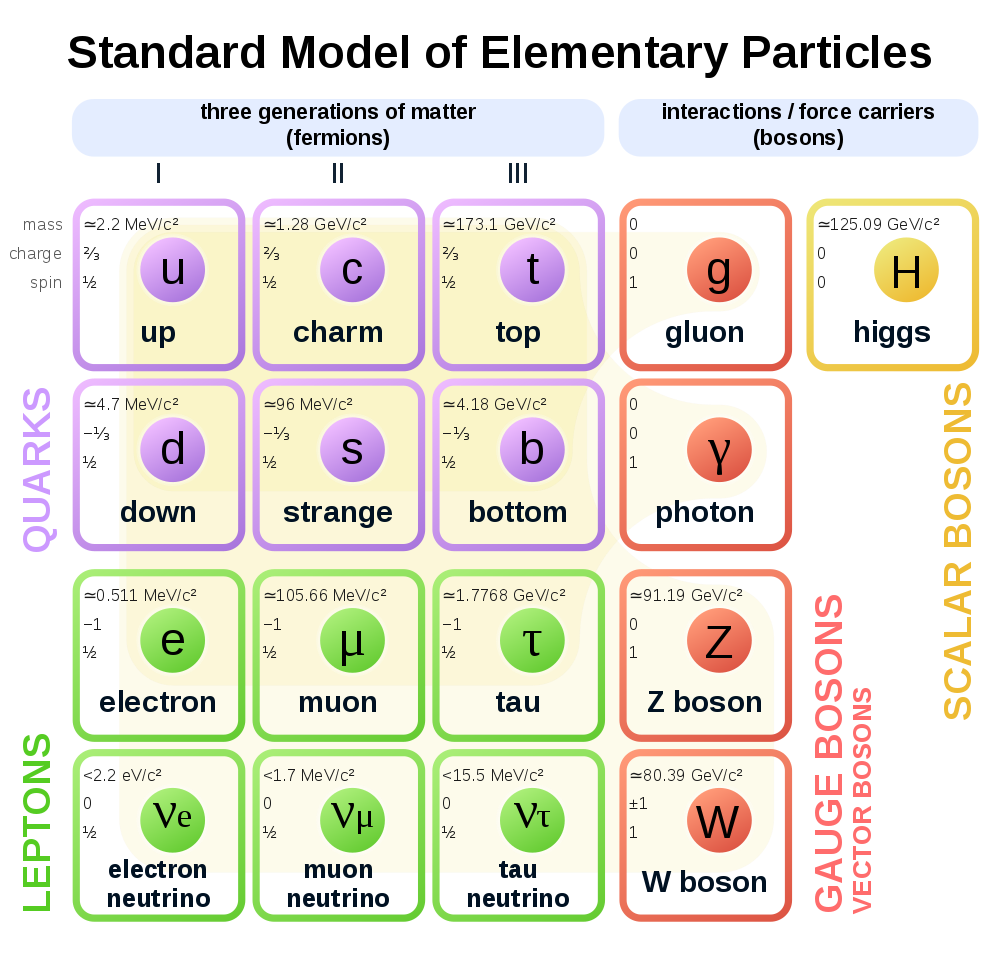
\includegraphics[width=0.7\linewidth]{img/theory/particles.png}
    \caption{
        Summary of the particles in the SM.
        % 
        The quarks, leptons, gauge bosons, and the Higgs boson are displayed in purple, green, red, and yellow cells, respectively.
        % 
        Each cell contains three numbers in the top-left corner, corresponding to the mass, electric charge, and spin of the particle.
        % 
        Taken from Ref.~\cite{particles-wikicommons}.
        }
    \label{fig:particles}
  \end{center}
\end{figure}




% ____________________________________________________________________________
\subsection{Quantum chromodynamics}
\label{sec:qcd}

\textit{%
The development of the theory of quantum chromodynamics has a fascinating history; at the time that quarks were first postulated by Gell-Mann and Zweig~\cite{griffiths}, there had been no experimental evidence for their existence at all.
% 
Only once deep inelastic electron-nucleon scattering became possible at sufficiently high energy to probe the internal structure of nucleons, the quark model was confirmed experimentally.
% 
This section starts from the full theory of QCD, loosely following the reasoning from Ref.~\cite{dissertori}, and mostly overlooks what was needed to develop it.
% 
For a historical overview of QCD the reader is referred to Refs.~\cite{dissertori,griffiths}. 
}


The SM Lagrangian for QCD is~\cite{dissertori}
% 
\begin{linenomath*}
\begin{equation}
\label{qcdlagrangian}
\lagrangian_\text{QCD} =
- \frac{1}{4} F^a_{\mu\nu} F^{a\mu\nu} 
+ \sum_\qquark \left( 
    \overline{\qquark}_i \mathrm{i} \gamma^\mu \delta_{ij} \partial_\mu \qquark_j
    - m_\qquark \delta_{ij} \overline{\qquark}_i \qquark_j
    - g_s \overline{\qquark}_i \gamma^\mu T_{ij}^a G_\mu^a \qquark_j
    \right)
\,,
\end{equation}
\end{linenomath*}
% 
where $\qquark$ ($\overline{\qquark}$) are the six (anti)quark fields, $\gamma$ are the gamma matrices, $m_\qquark$ is the quark mass, $F^a_{\mu\nu}$ is the gluon field strength tensor, $g_s$ is the coupling constant for QCD, $G^\mu$ are the gauge (gluon) fields, and $T^a$ are the generators of the SU(3) gauge symmetry group, which in the matrix representation equal $\lambda^a/2$, $\lambda_a$ being the Gell-Mann matrices.
% 
The field strength tensor is given by
% 
\begin{linenomath*}
\begin{equation}
F^a_{\mu\nu}
    = \partial_\mu G^a_\nu - \partial_\nu G^a_\mu - g_s f^{abc} G_\mu^b G_\mu^c
\,,
\end{equation}
\end{linenomath*}
% 
where $f^{abc}$ are the structure constants of the SU(3) symmetry group.
% 
The first, gluonic term of Equation~(\ref{qcdlagrangian}) is responsible for the gluon self-interactions, which consist of a vertex with three gluons and a vertex with four gluons---in contrast to electrodynamics, for which the gauge boson (i.e. the photon) has no self-interaction.
% 
The last term describes the interaction between quarks and gluons.


Besides the quark masses, the only free parameter in Equation~(\ref{qcdlagrangian}) is $g_s$.
% 
It is related to what is commonly referred to as the \textit{strong coupling constant of QCD} $\alphas$:
% 
\begin{linenomath*}
\begin{equation}
\as = \frac{g_s^2}{4\pi}
\,.
\end{equation}
\end{linenomath*}
% 
The corresponding solutions of the equation of motion for the QCD Lagrangian are obtained through perturbative expansion, i.e. \textit{perturbative QCD} (pQCD).
% 
In order for pQCD to converge, corrections need to decrease as one goes to higher orders, which requires small values of $\alphas$.
% 
As for the coupling in quantum electrodynamics, $\alphas$ is a running coupling that depends on the momentum transfer $Q$ of the process under consideration.
% 
As $g_s$ is a free parameter of the QCD Lagrangian, there exists no theoretical prediction for its value; however, once $\alphas$ is known at one value of $Q$, it can be calculated for any other value of $Q$ using the \textit{renormalization group equation} for QCD:
% 
\begin{linenomath*}
\begin{equation}
- Q^2 \frac{\partial\as}{\partial Q^2} = b_0 \as^2 + b_1 \as^3 + \mathcal{O}(\as^4)
\,,
\end{equation}
\end{linenomath*}
% 
where $b_0$ and $b_1$ are coefficients.
% 
Neglecting terms beyond $\mathcal{O}(\as^2)$ for a moment, the solution to the renormalization group equation becomes:
% 
\begin{linenomath*}
\begin{equation}
\as(Q^2) = \frac{1}{b_0 \ln \left( Q^2 / \Lambda_\text{QCD} \right)}
\,,
\end{equation}
\end{linenomath*}
% 
where $\Lambda_\text{QCD}$ is the scale at which the perturbative approximation no longer holds and non-perturbative effects become important.
% 
Evidently, the characterization of $\as(Q^2)$ is determined by the sign of $b_0$; if $b_0$ is negative, $\as(Q^2)$ diverges for large $Q$, if $b_0$ is positive for small $Q$.
% 
The coefficient $b_0$ is given by $(11 N_c - 2 N_f) / (12\pi)$~\cite{Dissertori:2015tfa}, where $N_c$ is the number of colors and $N_f$ is the number of flavors.
% 
In the SM, $b_0$ is positive, and as such $\alphas$ decreases with increasing $Q^2$, in stark contrast to the behavior of the coupling constant of quantum electrodynamics.
% 
This phenomenon is called \textit{asymptotic freedom}, and it is visualized in Fig.~\ref{fig:alphasscaling} together with measurements that confirm the expected scaling behavior.

\begin{figure}[hbtp]
  \begin{center}
    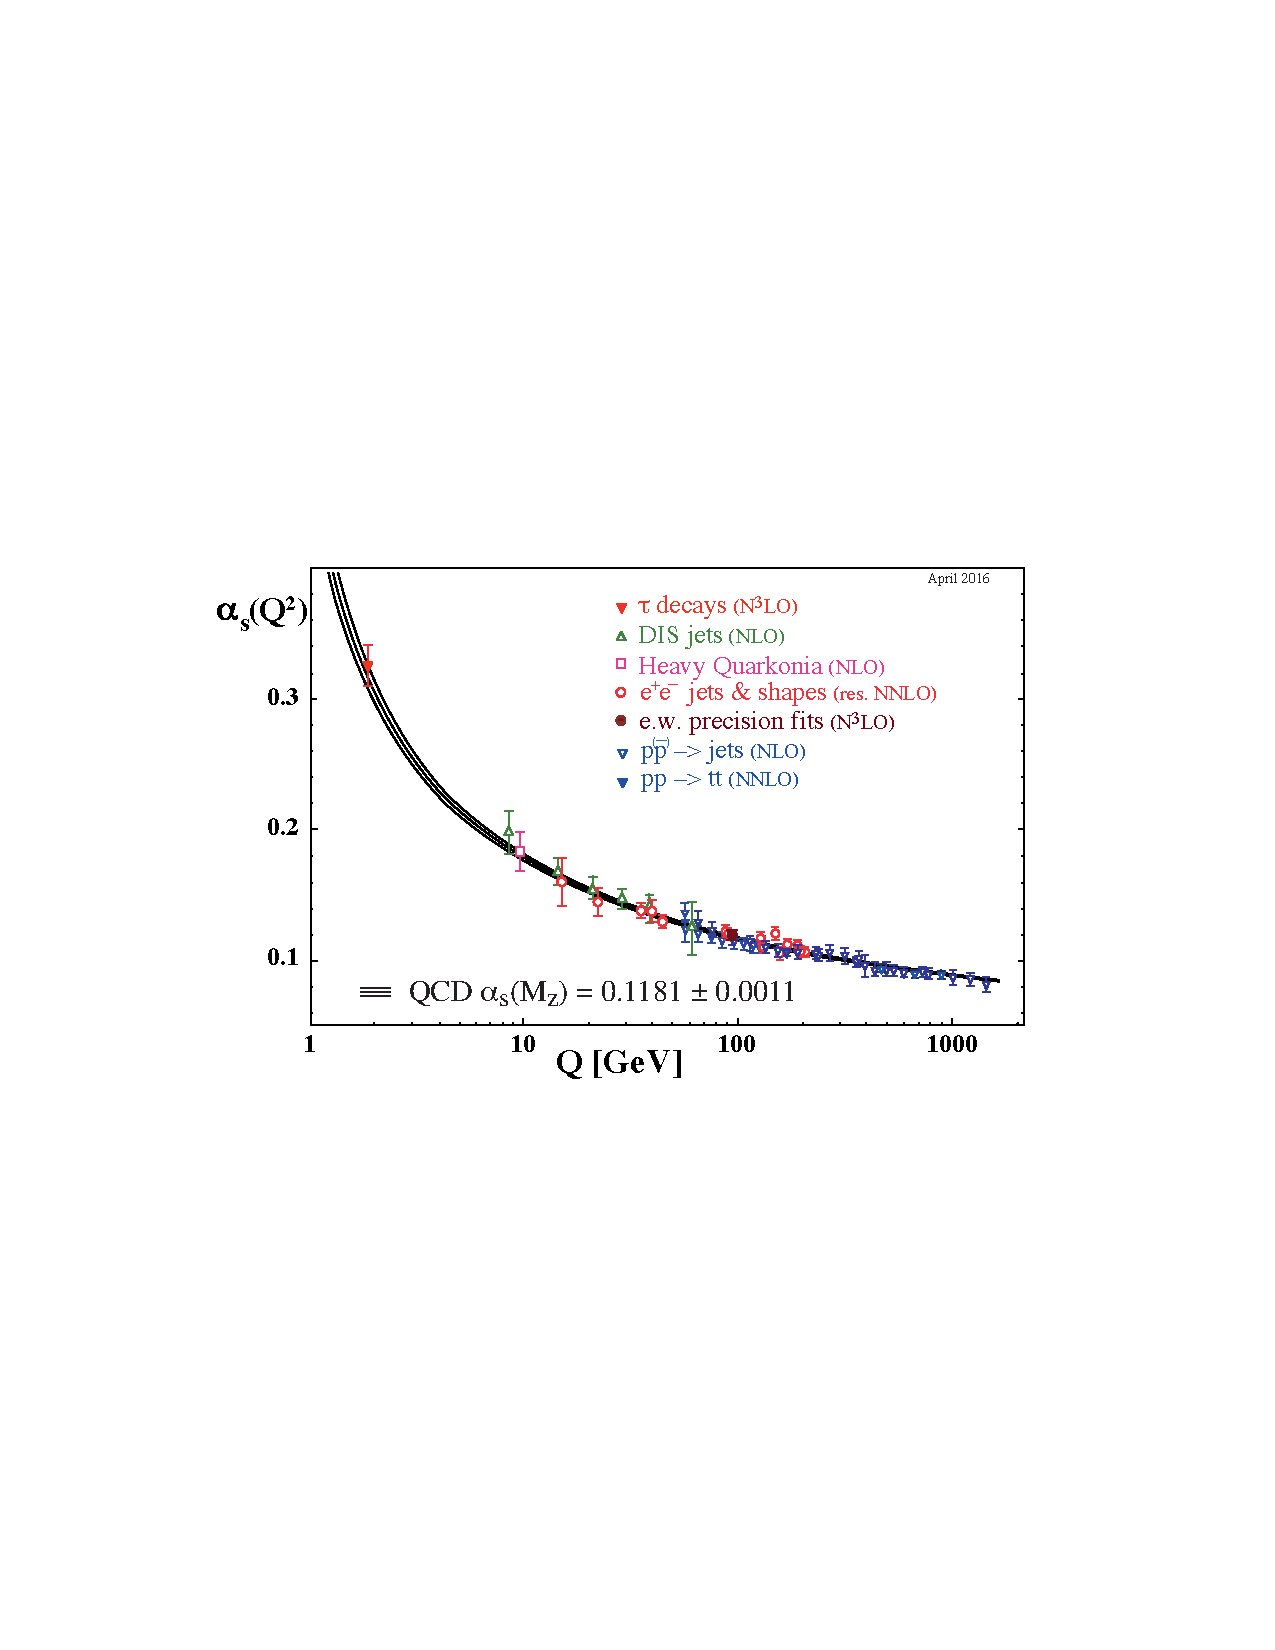
\includegraphics[width=0.7\linewidth]{img/theory/alphasscaling.pdf}
    \caption{
        Measurements of $\alphas(Q)$ at several values for $Q$.
        % 
        The black lines indicates the running of $\as(Q^2)$ when setting $\asmz$ to the current PDG world average~\cite{pdg}, plus or minus its uncertainty.
        % 
        Taken from Ref.~\cite{pdg}.
        }
    \label{fig:alphasscaling}
  \end{center}
\end{figure}



% ____________________________________________________________________________
\subsection{The Higgs mechanism}

Experimental observations undeniably point to massive $\wboson$ and $\zboson$ bosons, but including naive mass terms in the Lagrangian manifestly violates local gauge invariance.
% 
The Brout--Englert--Higgs mechanism~\cite{Higgs:1964pj,Englert:1964et,Guralnik:1964eu} was originally introduced as a solution to explain the massiveness of the vector bosons without violating gauge invariance.
% 
This section shortly illustrates the principle of the Higgs mechanism, closely following the reasoning found in Ref.~\cite{Djouadi:2005gi}.
% 
Rather than looking at the SM directly, consider a Lagrangian with a complex scalar field $\phi = \phi_\mathrm{R} + \imag \phi_\mathrm{C}$ coupled to a gauge field $A_\mu$ that resembles a photon in the QED Lagrangian:
% 
\begin{linenomath*}
\begin{equation}
\label{eq:lagrangian-higgs}
\lagrangian =
    -\frac{1}{4} F_{\mu\nu} F^{\mu\nu}
    + (\partial^\mu - \imag e A^\mu) \phi^\ast (\partial_\mu + \imag e A_\mu) \phi
    - \underbrace{(\mu^2 \phi^\ast \phi + \lambda (\phi^\ast \phi)^2)}_{V(\phi)}
\,,
\end{equation}
\end{linenomath*}
% 
where $F_{\mu\nu} = \partial_\mu A_\nu - \partial_\nu A_\mu$ and $V(\phi)$ is a potential that yields a self-interaction for $\phi$.
% 
It can be easily verified that this Lagrangian is invariant under the transformations
% 
\begin{linenomath*}
\begin{equation}
\label{eq:transformations-higgs}
\phi(x) \to \exp{\imag \alpha(x)} \phi(x)
\quad \text{and} \quad 
A_\mu(x) \to A_\mu(x) - \frac{1}{e} \partial_\mu \alpha(x)
\,.
\end{equation}
\end{linenomath*}
% 
For $\mu > 0$, the term $\mu^2 \phi^\ast \phi$ is a regular mass term; the Lagrangian describes simply a `charged' scalar particle of mass $\mu$ and an `electromagnetic' field $A_\mu$, much like the QED Lagrangian for a complex scalar field except a $(\phi^\ast\phi)^2$ self-interaction is added.
% 
For $\mu < 0$, the minimum of the potential, found by solving $\partial V / \partial \phi = 0$, yields:
% 
\begin{linenomath*}
\begin{equation}
\left< 0 | \phi^\ast\phi | 0 \right> = \frac{-\mu^2}{2\lambda}  \equiv  \frac{v^2}{2}
\quad \left( \text{with} \; v = \sqrt{\frac{-\mu^2}{\lambda}} \right)
\end{equation}
\end{linenomath*}
% 
and the vacuum expectation value, $\left< 0 | \phi | 0 \right>$, becomes non-zero:
% 
\begin{linenomath*}
\begin{equation}
\left< 0 | \phi | 0 \right> = \sqrt{ \frac{-\mu^2}{2\lambda} } = \frac{v}{\sqrt{2}}
\,.
\end{equation}
\end{linenomath*}
% 
Clearly the Lagrangian can no longer be interpreted as that of a particle of mass $\mu$.
% 
In order to rewrite the Lagrangian so that the physical interpretation of massive particles is restored, $\phi$ is expanded around the vacuum expectation value:
% 
\begin{linenomath*}
\begin{equation}
\label{eq:expansion-around-minimum}
\phi = \frac{1}{\sqrt{2}} \left( v + \phi_1(x) + \imag \phi_2(x) \right)
\,.
\end{equation}
\end{linenomath*}
% 
Using the gauge transformations in Equation~(\ref{eq:transformations-higgs}) and a clever choice of $\alpha(x)$, the imaginary part of this expansion can be set to $0$:
% 
\begin{linenomath*}
\begin{equation}
\phi = \frac{1}{\sqrt{2}} \left( v + \phi_1(x) + \imag \phi_2(x) \right)
\to
\phi^\prime = \exp{i\alpha(x)} \frac{1}{\sqrt{2}} \left( v + \phi^\prime_1(x) \right)
\,.
\end{equation}
\end{linenomath*}
% 
As we will not use the untransformed fields any further, from here on the prime is omitted from $\phi_1^\prime$.
% 
The expansion is then inserted into the Lagrangian in Equation~(\ref{eq:lagrangian-higgs}).
% 
Performing the substitution is straightforward but lengthy; the derivation is given in Appendix~\ref{app:theory}, and here only the result is given:
% 
\begin{linenomath*}
\begin{equation}
\lagrangian \to \lagrangian^\prime =
    -\frac{1}{4} F_{\mu\nu} F^{\mu\nu}
    + \frac{1}{2} \partial^\mu \phi_1 \partial_\mu \phi_1
    + \frac{1}{2} e^2 (v+\phi_1)^2 A^\mu A_\mu
    - \frac{1}{4}\lambda\phi_1 - v\lambda\phi_1^3 + \mu^2\phi_1^2 - \frac{1}{4}\mu^2 v^2
\,.
\end{equation}
\end{linenomath*}
% 
The first two terms of the transformed Lagrangian look similar to the untransformed case.
% 
Additionally, there are $\phi_1^3$ and $\phi_1^4$ interactions, a constant term which is of no importance, and a mass term for $\phi_1$ that corresponds to particle of mass $-2\mu$.
% 
Expanding the third term yields the interactions between $\phi_1$ and $A_\mu$, but importantly, it also yields a term $\frac{1}{2}e^2v^2 A^\mu A_\mu$; this then is the mass term for $A_\mu$.
% 
The transformations described in Equation~(\ref{eq:transformations-higgs}) are clearly not valid if applied analogously to the fields in this transformed Lagrangian; the symmetry that was present before the transformation is `broken'.


Spontaneous symmetry breaking in the SM Lagrangian is conceptually not different from the above demonstration, but significantly lengthier and slightly more complicated.
% 
Instead of a single complex scalar field, one considers a complex doublet of scalar fields, and carefully picks the vacuum around which to expand so the $U(1)$ symmetry of QED is preserved.
% 
The derivation of the transformed Lagrangian can be found in Ref.~\cite{Djouadi:2005gi}.
% 
In the end one finds massive $\zboson$ and $\wboson$ bosons, a massless photon, and a massive Higgs boson, with triple and quartic self-interactions much like in the derivation above.
% 
Also the fermion masses can be explained through the Higgs mechanism, and in the SM it turns out the fermion mass is proportional to the coupling of the Higgs boson with the respective fermion.
% 
As can be seen in Fig.~\ref{fig:massproportion}, this not particularly trivial finding is thus far in good agreement with the observations; the proportionality of the Higgs boson couplings to the particle masses holds well over scales that vary over many order of magnitudes.
% 
Although the Higgs mechanism incorporates masses into the SM Lagrangian beautifully, the actual values of the masses still need to be determined experimentally.


\begin{figure}[hbtp]
  \begin{center}
    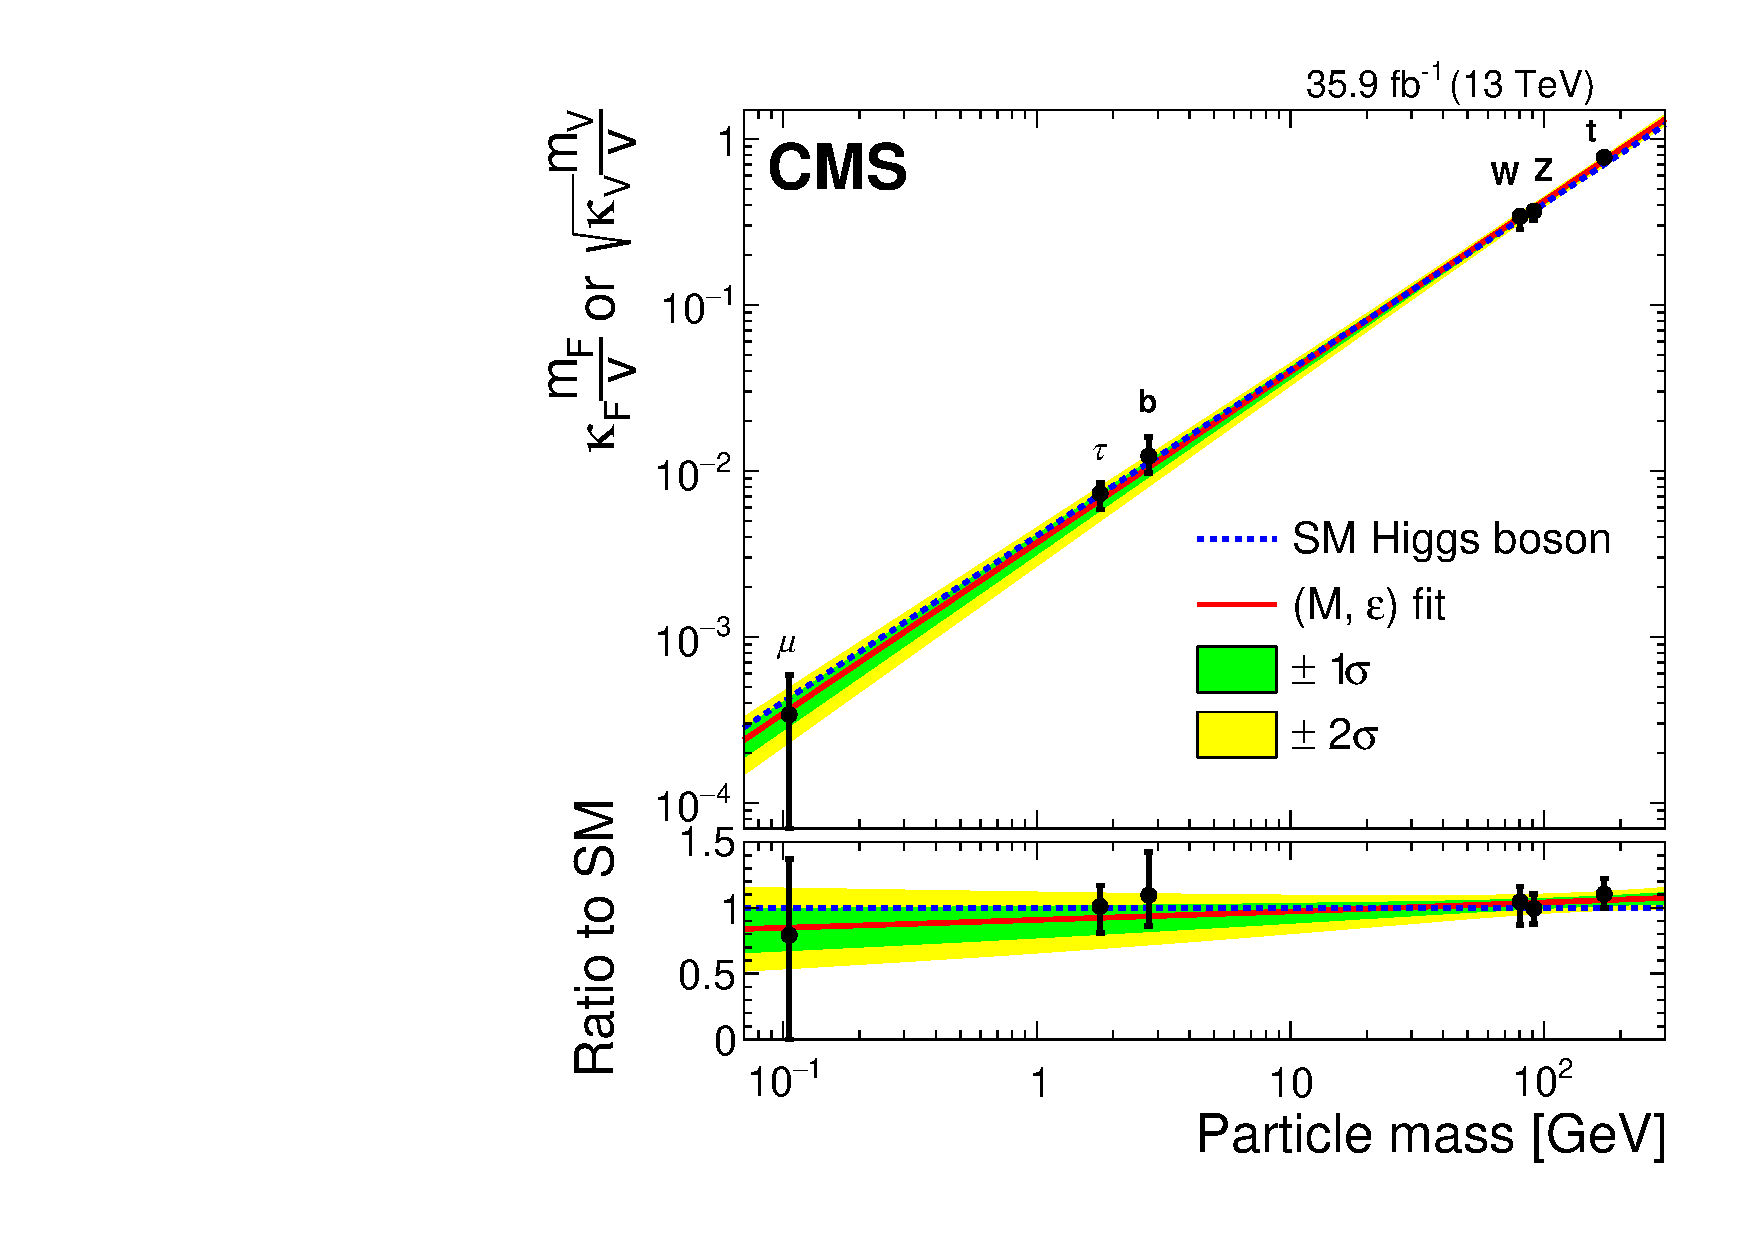
\includegraphics[width=\halflinewidth]{img/theory/grandcomb/massproportion.pdf}
    \caption{
        Observed Higgs boson couplings as a function of the corresponding particle masses, with the SM shown as a black dotted line.
        % 
        Taken from Ref.~\cite{Sirunyan:2018koj}.
        }
    \label{fig:massproportion}
  \end{center}
\end{figure}


% ____________________________________________________________________________
\subsection{Higgs boson production modes and decay channels}
\label{sec:production-decay}

The formulas for the production modes and decay channels described below all assume a SM Higgs boson.
% 
The resonance discovered in 2012 has so far proven to be consistent with the SM Higgs boson, but this consistency is under constant scrutiny.
% 
A convenient framework to evaluate the likeliness of the $125$\GeV resonance to be the SM Higgs boson is the \textit{\kappaframework}~\cite{LHCHXSWG:YR3}, in which the SM couplings of the Higgs boson with other particles are modified as:
% 
\begin{linenomath*}
\begin{equation}
\kappa_{i} = \frac{y_{i}}{y_{i}^{\text{SM}}}\,,
\end{equation}
\end{linenomath*}
% 
where $y_i$ is the Higgs boson coupling to particle $i$, and $\kappa_i$ is the corresponding \textit{coupling modifier}, which will often also be referred to as simply `the coupling'.
% 
The SM value of any $\kappa_i$ is equal to 1.
% 
The coupling modifiers naturally affect the production as well as the decay of the Higgs boson, and whenever one tests the SM by interpreting data in terms of coupling modifiers, one has to be careful to treat both production and decay appropriately.


The Higgs boson production and decay is possible through a myriad of modes and channels, and most of them are relevant in the context of hadron colliders.
% 
As the rest of this thesis is concerned with Higgs boson couplings, also the scaling of the production modes and decay channels in terms of Higgs boson couplings is discussed briefly.
% 
The Higgs boson is produced at hadron colliders through the following production modes (sorted by decreasing production cross section):
% 
\begin{itemize}
\item \textit{Gluon fusion} (\ggh), which in the SM exists only via a loop of (usually heavy) particles that couple to the Higgs boson, as the direct coupling of the Higgs boson to the gluon field is zero in the SM;
% 
\item \textit{Vector boson fusion} (\vbf), in which the Higgs boson is radiated off a virtual vector boson; the final state is characterized by two jets in the forward and backward regions;
% 
\item \textit{Associated production with a vector boson} (\vh), in which the Higgs boson is radiated off a vector boson;
% 
\item \textit{Associated production with top quarks} (\tth), in which the Higgs boson is radiated off a top quark; and
% 
\item \textit{Associated production with bottom quarks} (\bbh), in which the Higgs boson is radiated off a bottom quark.
\end{itemize}
% 
The leading order diagrams for these production modes are shown in Fig.~\ref{fig:productionmodes}.
% 
The $\ggh$ production mode is dominant at the LHC, and its scaling in terms of Higgs boson couplings is complicated by interference terms of the loop constituents.
% 
The $\tth$ and $\bbh$ production modes contain at leading order a single quark-Higgs boson vertex, which results in a simple quadratic dependence on the Higgs boson couplings for the respective production cross sections.


\begin{figure}[hbtp]
  \begin{center}
    % \includegraphics[width=0.7\linewidth]{img/theory/productiondiagrams_combined.png}
    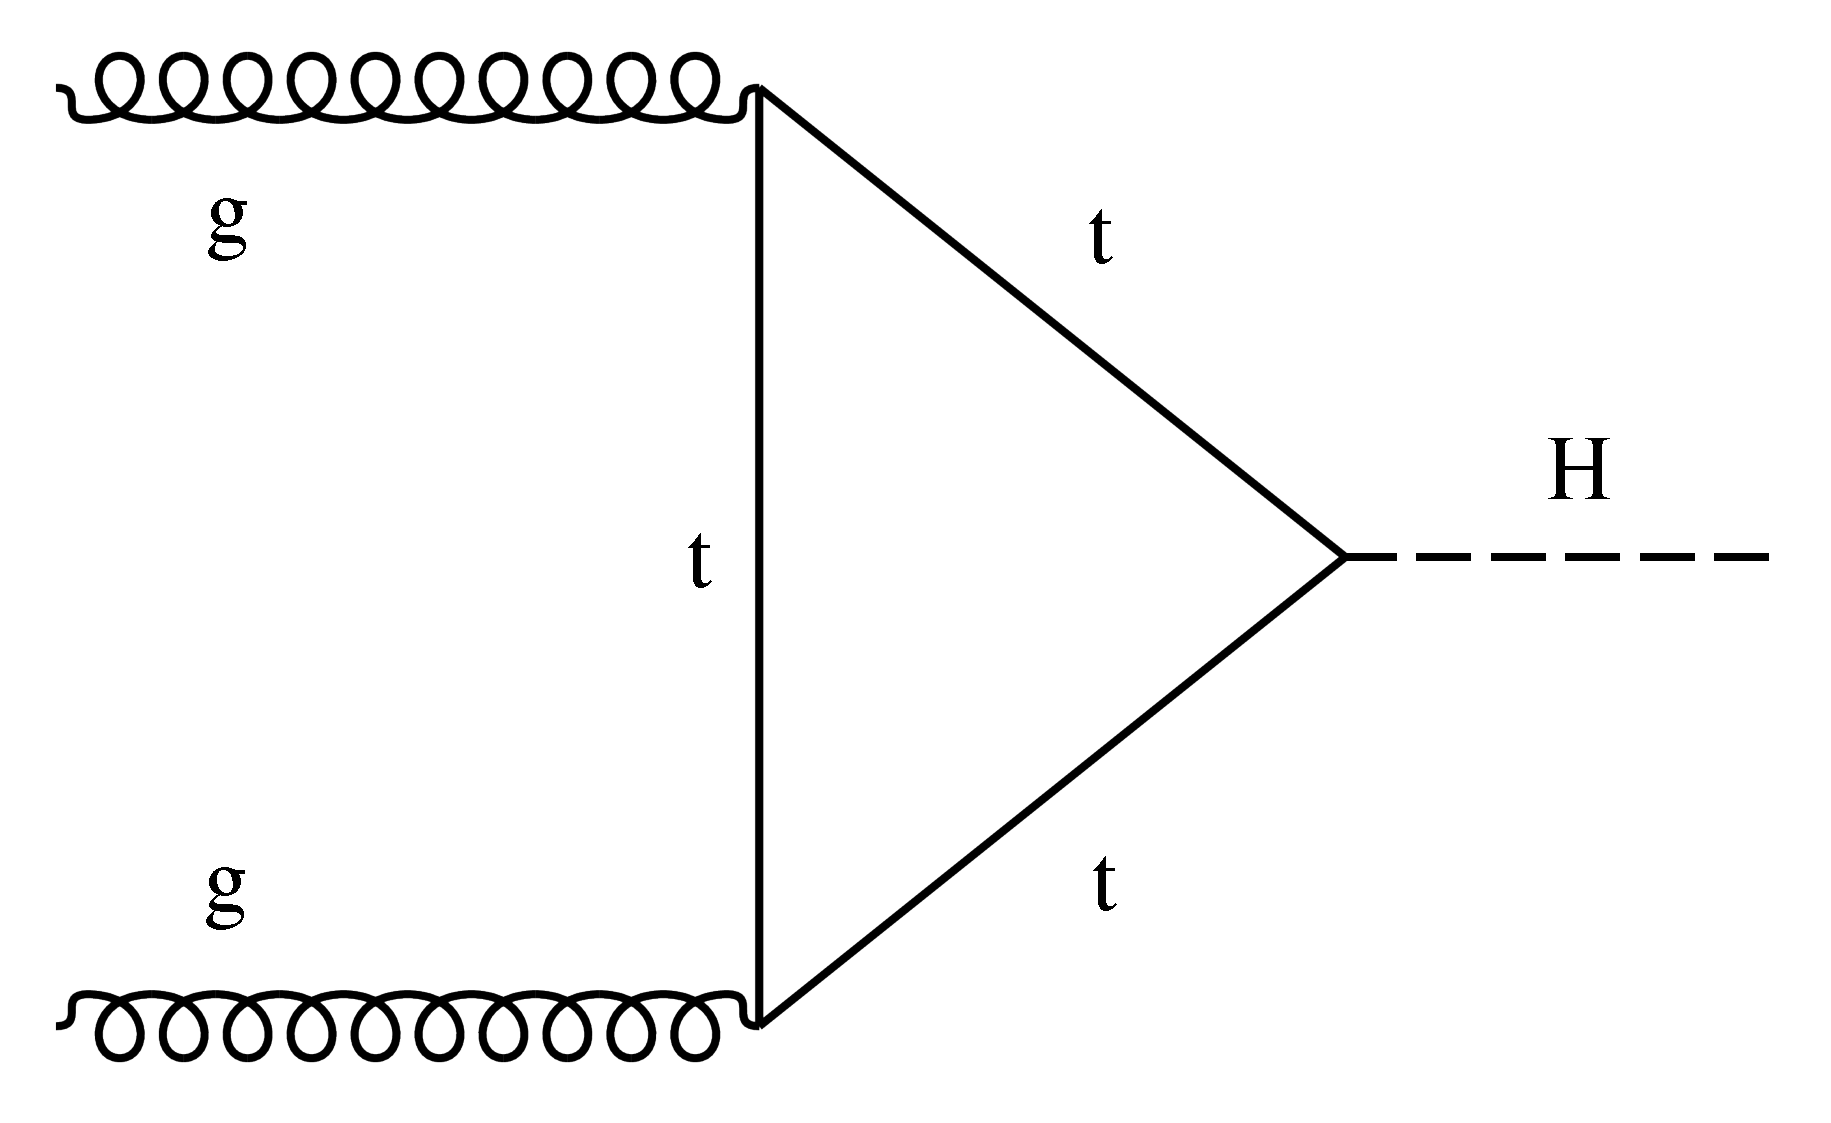
\includegraphics[width=0.35\linewidth]{img/theory/grandcomb/ggh.pdf}
    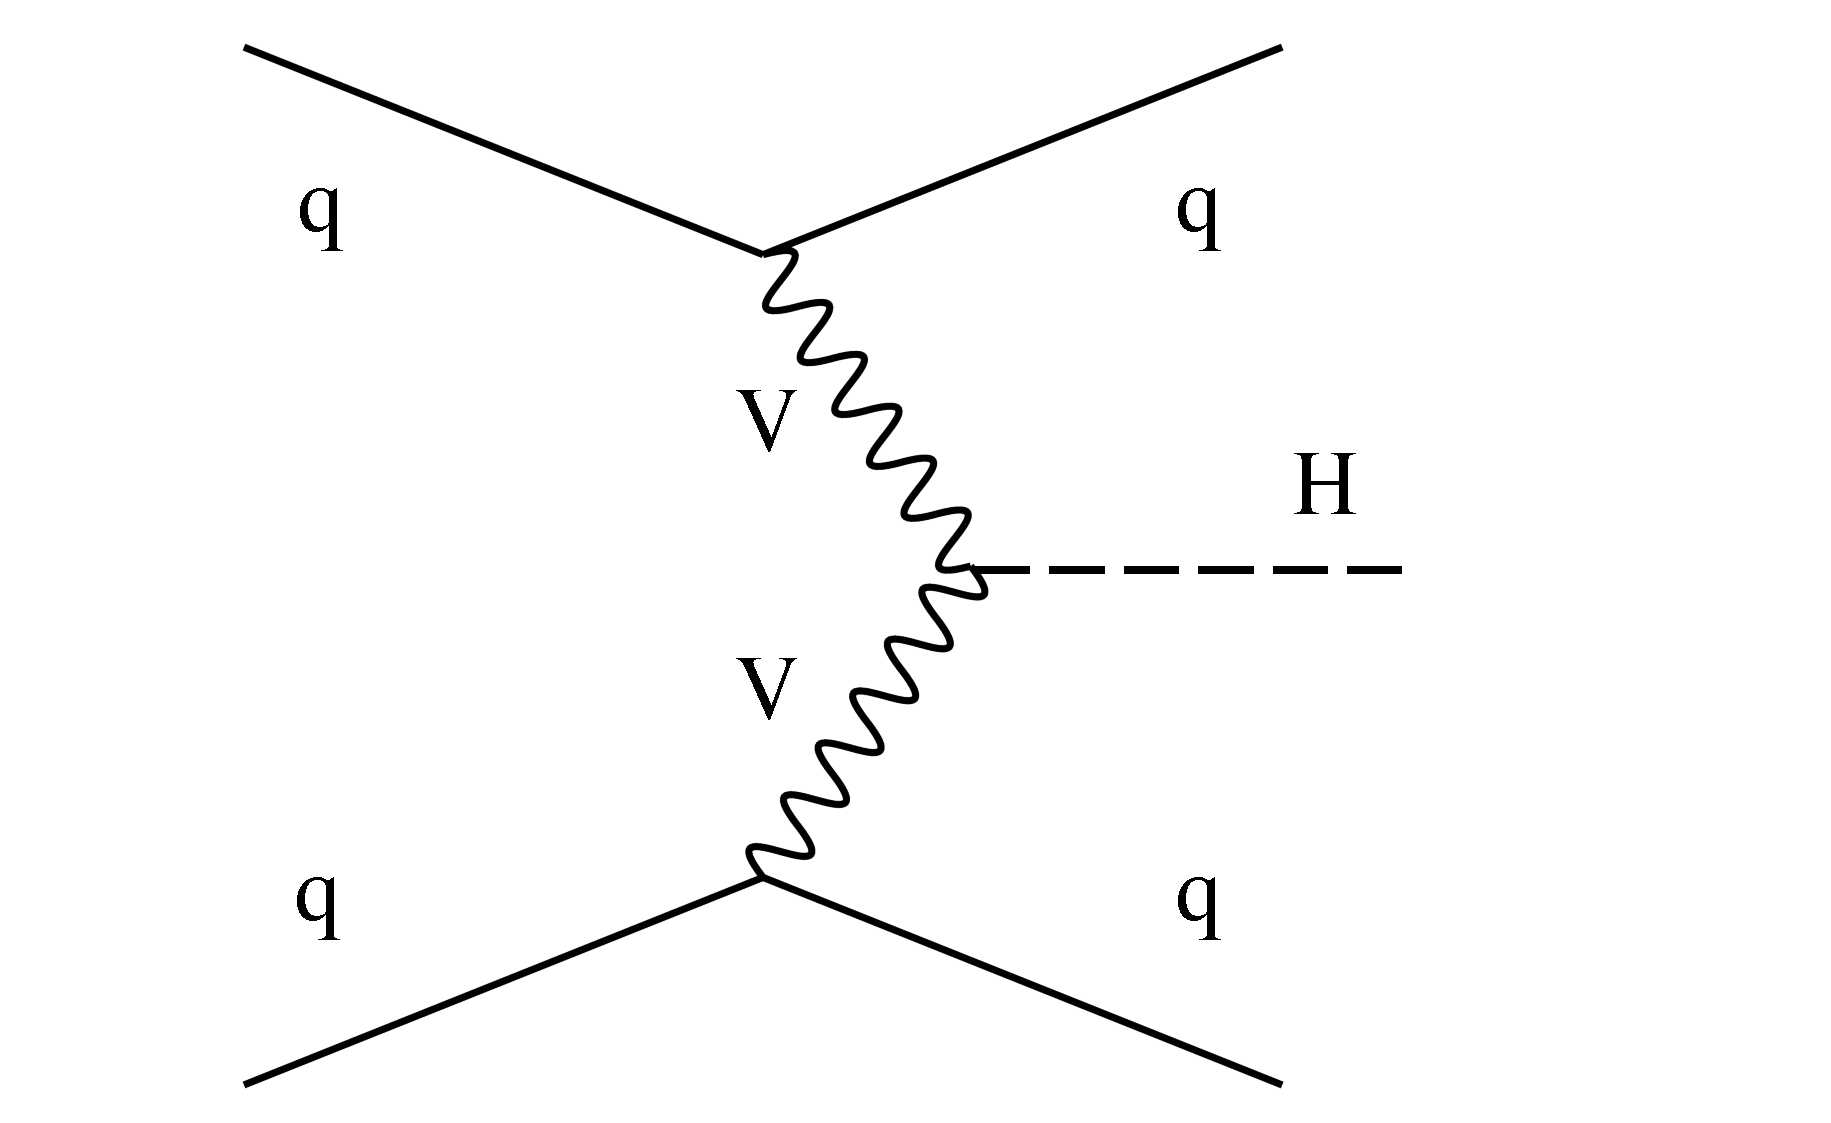
\includegraphics[width=0.35\linewidth]{img/theory/grandcomb/vbf.pdf}
    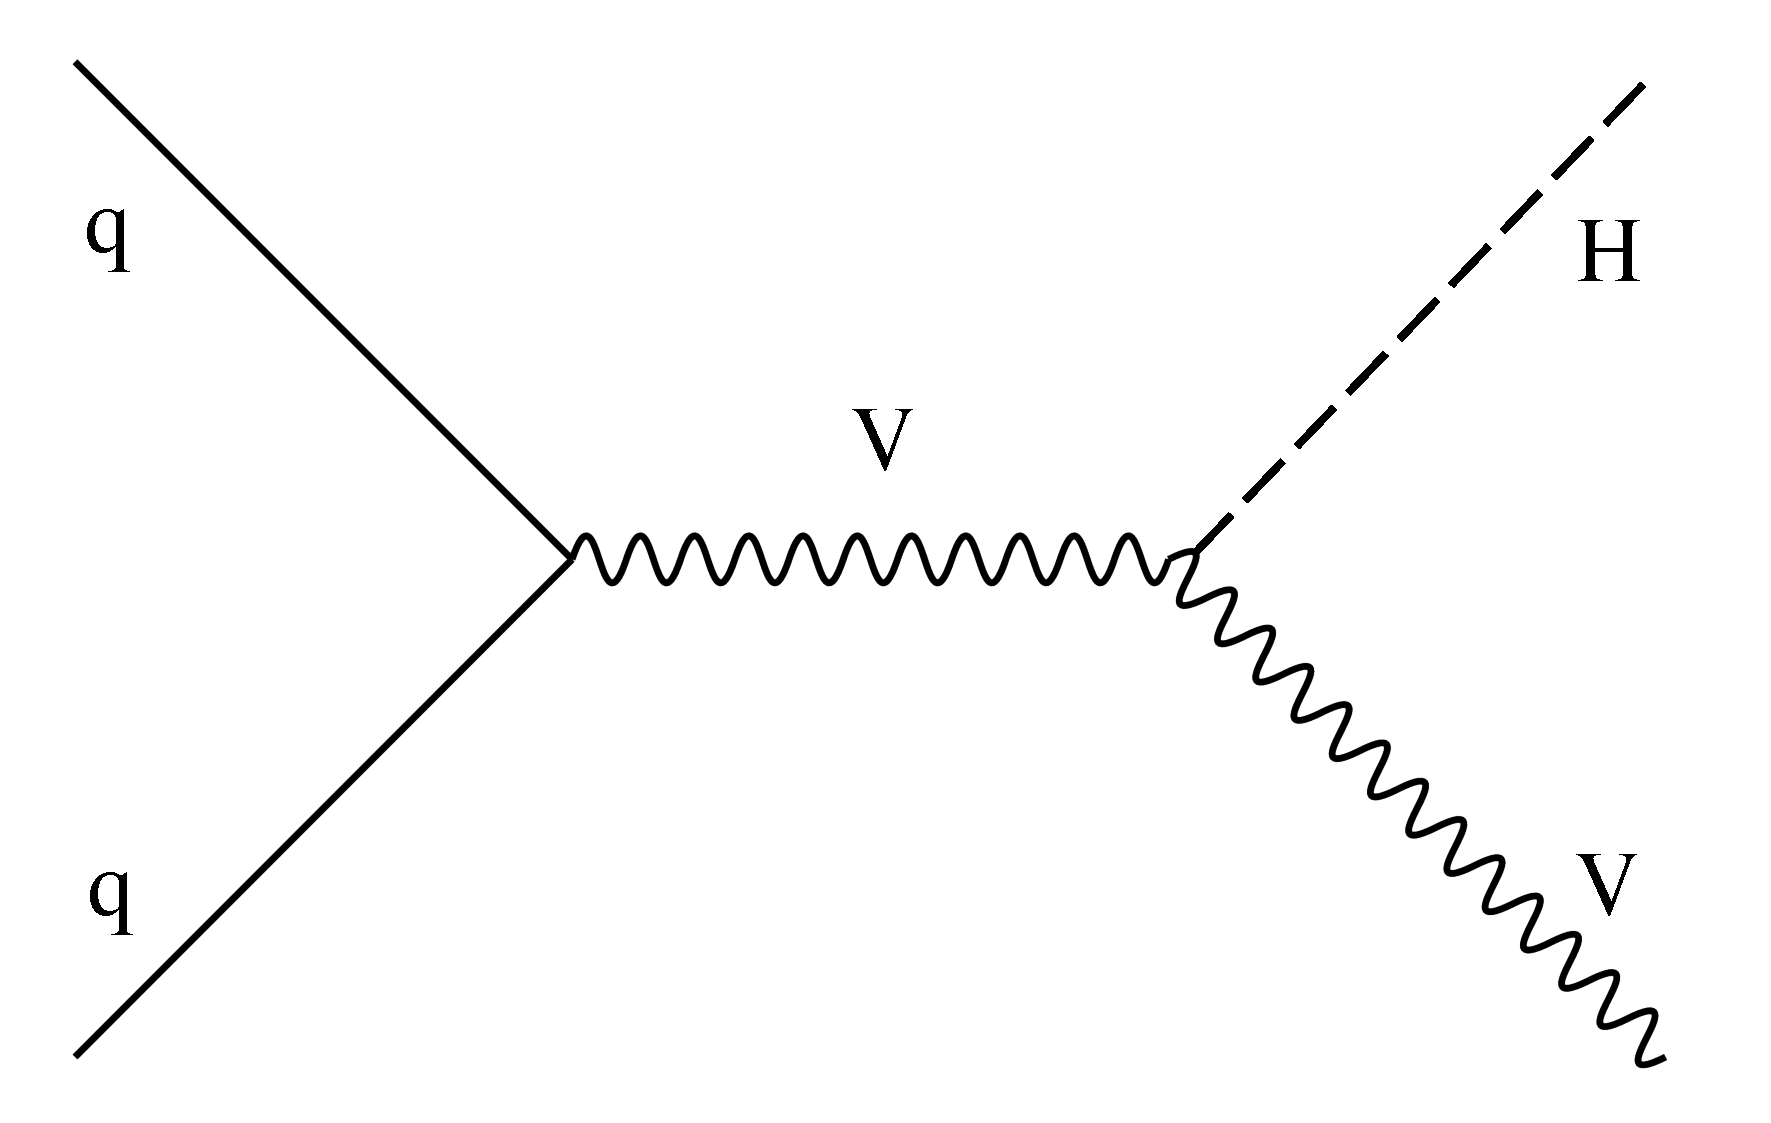
\includegraphics[width=0.35\linewidth]{img/theory/grandcomb/vh.pdf}
    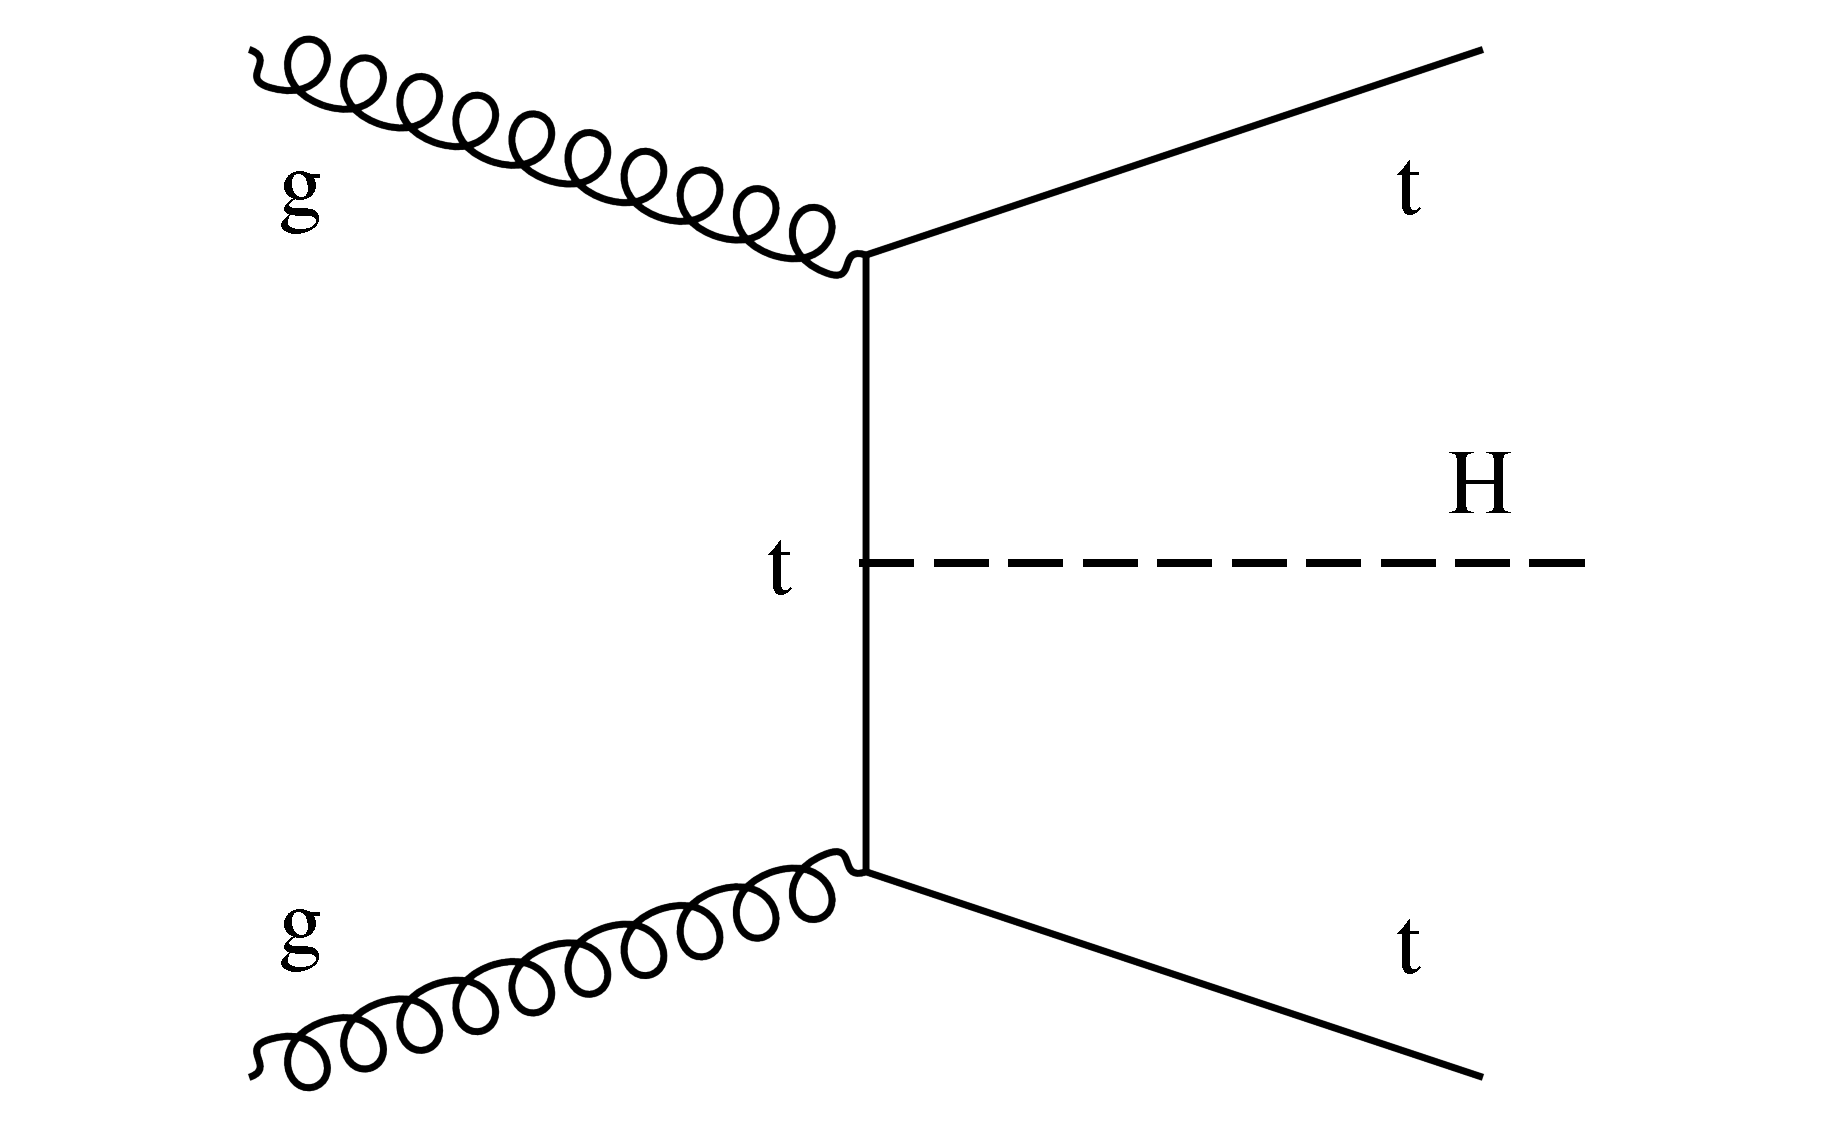
\includegraphics[width=0.35\linewidth]{img/theory/grandcomb/tth.pdf}
    \caption{
        Summary of the dominant Higgs boson production modes at hadron colliders: $\ggh$ (top left), $\vbf$ (top right), $\vh$ (bottom left), and $\tth$ (bottom right).
        % 
        The $\bbh$ production mode has the same leading order diagram as $\tth$, but with the top quarks replaced by bottom quarks.
        % 
        Taken from Ref.~\cite{Sirunyan:2018koj}.
        }
    \label{fig:productionmodes}
  \end{center}
\end{figure}


The Higgs boson decay channels are slightly more numerous.
% 
The most common decay channels without a loop are the decays to two $\zboson$ bosons ($\hzz$), two $\wboson$ bosons ($\hww$), two $\taulepton$ leptons ($\htautau$), two $\bquark$ quarks ($\hbb$), and two $\cquark$ quarks ($\hcc$).
% 
The decay widths of these channels all scale quadratically with respect to their SM decay widths in terms of their respective coupling to the Higgs boson, e.g. $\Gamma(\hbb) / \Gamma(\hbb)_\text{SM} = \kappab^2$.
% 
For the fermions, the decay width is given by (excluding QCD corrections in the case of quarks)~\cite{higgshunter}
% 
\begin{linenomath*}
\begin{equation}
\label{eq:brhff}
\Gamma(\hboson \to f\overline{f})
=
\frac{N_c g^2 m_f^2}{32\pi m_\wboson^2}
\left( 1-4\frac{m_f^2}{\mh^2} \right)^{ 3/2 }
\mh 
\,,
\end{equation}
\end{linenomath*}
% 
where $g$ is the electroweak coupling constant.
% 
The decay width becomes larger for heavier fermions, with the kinematically not accessible exception of the decay width to two top quarks.
% 
% Since the Higgs boson-fermion couplings are proportional to the fermion mass, the decay width is typically larger for heavier fermions, with the obvious exception of the decay width to two top quarks.
% 
In practice, the decay width to quarks lighter than the charm is negligible, as well as the decay width to two electrons.
% 
The leading-order decay widths to vector bosons are given by~\cite{higgshunter}
% 
\begin{linenomath*}
\begin{equation}
\Gamma(\hzz)
=
\frac{g^2}{128\pi} \frac{\mh^3}{m_\wboson^2}
\sqrt{1-x_\zboson}
\left( 1 - x_\zboson + \frac{3}{4} x_\zboson^2 \right)
\,
\end{equation}
\end{linenomath*}
% 
for the $\hzz$ channel, and
% 
\begin{linenomath*}
\begin{equation}
\Gamma(\hww)
=
\frac{g^2}{64\pi} \frac{\mh^3}{m_\wboson^2}
\sqrt{1-x_\wboson}
\left( 1 - x_\wboson + \frac{3}{4} x_\wboson^2 \right)
\,
\end{equation}
\end{linenomath*}
% 
for the $\hww$ channel, where $x_{\zboson \, (\wboson)} = 4 m_{\zboson\,(\wboson)}^2 / \mh$.


Besides decays involving a single vertex, the Higgs boson decays via loops to two photons ($\hgg$), two gluons ($\hgluglu$), and a photon and a $\zboson$ boson ($\hzg$).
% 
In these cases the decay width calculation needs to take interference terms into account.
% 
For example, in the case of $\hgg$, the decay width is given by~\cite{higgshunter}
% 
\begin{linenomath*}
\begin{equation}
\Gamma(\hgg) =
\frac{\alpha^2g^2}{1024\pi^3} \frac{\mh^3}{m_\wboson^2}
\left|
\sum_{i,j} N_{cj} e_j^2 F_i^j
\right|^2
\,,
\end{equation}
\end{linenomath*}
% 
where $i$ is an index to spin-0, spin-1/2 or spin-1, $e_j$ is the electromagnetic charge  for particle $j$, $N_c^j$ is the number of colors (i.e. only 3 for quarks, otherwise 1), and $F_i^j$ is given by
% 
\begin{linenomath*}
\begin{equation}
\begin{split}
F_0^j     &= \tau (1- \tau f(\tau)) \\
F_{1/2}^j &= 2\tau ( 1 + (1-\tau) f(\tau) ) \\
F_1^j     &= 2 + 3\tau + 3\tau( 2-\tau ) f(\tau)
\,,
\end{split}
\end{equation}
\end{linenomath*}
% 
with $\tau = 4m_j^2/\mh^2$ and
% 
\begin{linenomath*}
\begin{equation}
\label{eq:ffunction}
f(\tau) = \left\{% This will break the tex parser!!!
\begin{array}{ll}
\left( \text{sin}^{-1}\left(\sqrt{1/\tau}\right) \right)^2 ,
    & \quad \text{if} \; \tau \ge 1, \\[9pt]
-\frac{1}{4} \left(
        \ln \left(\frac{1+\sqrt{1-\tau}}{1-\sqrt{1-\tau}} \right)
        -\imag \pi 
        \right)^2
    & \quad \text{if} \; \tau < 1.
\end{array}%
\right. 
\end{equation}
\end{linenomath*}
% 
For the decay channels involving a loop, the scaling with respect to the Higgs boson couplings is more complicated due to the interference terms.
% 
In the case of $\hgg$, the scaling is approximately given by~\cite{higgshunter}
% 
\begin{linenomath*}
\begin{equation}
\frac{\Gamma(\hgg)}{\Gamma(\hgg)_\text{SM}} \approx
        7.15 \times 10^{-2}    \;   \kappat^2
        % + 1.94 \times 10^{-5}   \kappab^2
        + 1.59                \;  \kappaw^2
        % - 1.77 \times 10^{-3}     \kappat\kappab
        - 6.74 \times 10^{-1} \;  \kappat\kappaw
        % + 8.35 \times 10^{-3}   \kappab\kappaw
\,,
\end{equation}
\end{linenomath*}
% 
where the interference with lighter particles in the loop has been neglected.
% 
The decay widths of the $\hgluglu$ and $\hzg$ channels and their scaling in terms of Higgs boson couplings can be found in Ref.~\cite{higgshunter}.
% 
The branching fractions are given by the ratio of the corresponding decay width over the sum of all decay widths.


Equations~(\ref{eq:brhff}-\ref{eq:ffunction}) indicate that the branching fractions depend rather strongly on $\mh$; although not explicitly shown in this section, the same is true for the production cross sections.
% 
Figure~\ref{fig:mh-production-decay} shows the production cross sections (left) and branching fractions (right) as a function of $\mh$.
% 
At the SM value of the Higgs mass, around 125\GeV~\cite{Aad:2015zhl}, the dominant production mechanism is $\ggh$, and the most common decay channel is $\hbb$.

\begin{figure}[hbtp]
  \begin{center}
    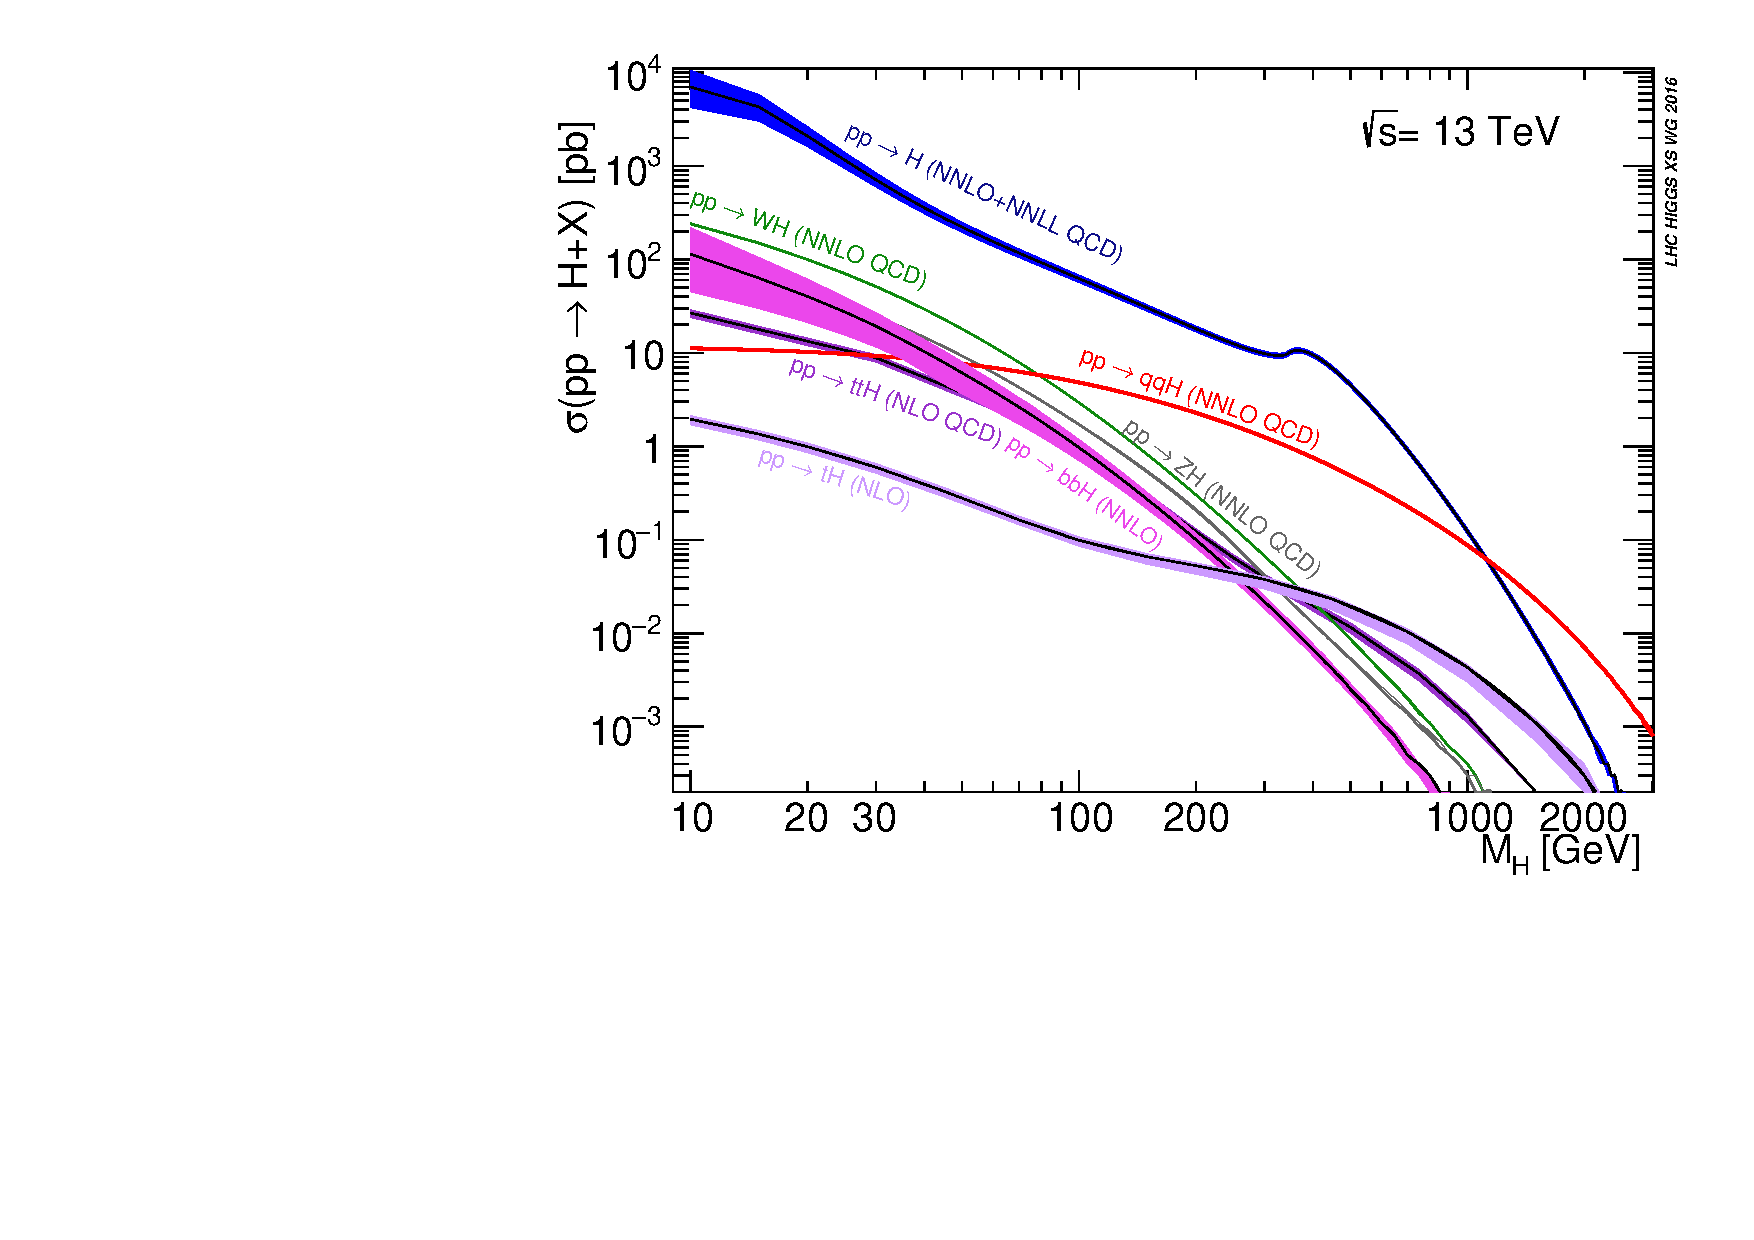
\includegraphics[width=\halflinewidth]{img/theory/mh_production.pdf}
    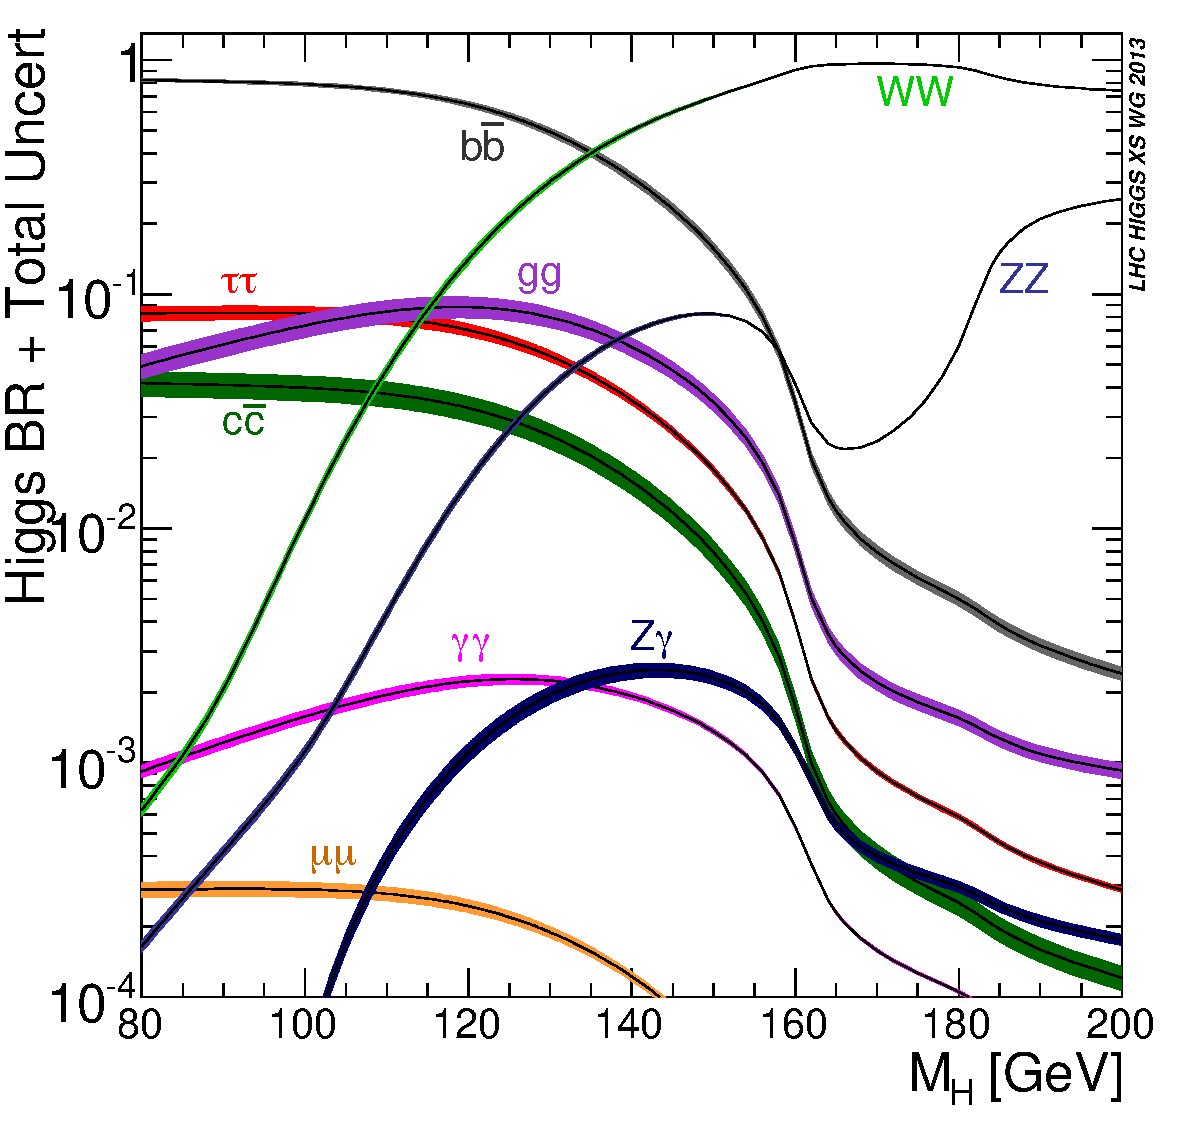
\includegraphics[width=\halflinewidth]{img/theory/mh_decay.pdf}
    \caption{
        Higgs boson production cross sections for several production modes as a function of $\mh$ (left, taken from Ref.~\cite{deFlorian:2016spz}) and branching fractions for several decay channels (right, taken from Ref.~\cite{LHCHXSWG:YR3}).
        }
    \label{fig:mh-production-decay}
  \end{center}
\end{figure}



% ____________________________________________________________________________
\subsection{The transverse momentum spectrum}
\label{sec:theory-pt}

The predictions of differential distributions are determined primarily by the predictions of $\ggh$, the dominant Higgs boson production mode at the LHC.
% 
Because of the loop in the LO $\ggh$ diagram, the $\pth$ distribution of Higgs bosons produced via $\ggh$ is a good probe for new physics and a portal towards precision measurements of the Higgs boson properties, for multiple reasons.
% 
Firstly, up until now, finite quark mass effects in the $\pth$ spectrum have not been observed experimentally; only now sufficient data is collected, and confirming these effects is an important verification of the SM.
% 
Secondly, the couplings of the Higgs boson to other SM particles can affect the shape of differential distributions while preserving the overall normalization~\cite{Bishara:2016jga,Grazzini:2017szg,Grazzini:2016paz}.
% 
By fitting the shape of theoretical predictions under simultaneous variations of Higgs boson couplings to the shape observed in data, the Higgs boson couplings can be further constrained.
% 
And thirdly, if there any heavy beyond-the-SM particles in the loop, the tails of the $\pth$ are expected to deviate with respect to their SM values~\cite{Banfi:2013yoa}.
% 
As the tails concern only a small part of the inclusive cross section, these deviations would be hard to observe in an inclusive cross section measurement.
% 
The interpretation performed in Section~\ref{sec:interpretation} is concerned with the first two points, although the applied methodology would as well be suitable for a search of heavy particles in the $\ggh$ loop.


As this thesis is concerned primarily with the interpretation of the $\pth$ spectrum, this section shortly introduces the main aspects of its calculation and the most recently obtained results.
% 
The transverse momentum can be written in terms of the Mandelstam variables $s$, $u$, and $t$~\cite{peskin}:
% 
\begin{linenomath*}
\begin{equation}
\pt^2 = \frac{u \, t}{s}
\,.
\end{equation}
\end{linenomath*}
% 
The matrix element can be calculated in terms of the Mandelstam variables, and then expressed as a differential cross section of $\pt$.
% 
% , yielding the transverse momentum spectrum.
% 
In the case of $\ggh$, the transverse momentum of the Higgs boson originates from QCD radiation---e.g. from the radiation of a single gluon ($\gluon\gluon\to\hboson\gluon$)---the contribution of which appears beyond the leading-order calculation.
% 
The lowest-order differential cross sections of Higgs boson production via $\ggh$ were first calculated in Ref.~\cite{Ellis:1987xu}; assuming an infinite top quark mass (called the \textit{heavy top mass limit} $\mt \gg \mh$, abbreviated as HTL), one finds the following expression:
% 
\begin{linenomath*}
\begin{equation}
\frac{\mathrm{d}\sigma}{\mathrm{d}t} =
\frac{1}{16\pi s^2} \frac{1}{4v^2}
\sum_\text{spins, colors} \abs{\mathcal{M}}^2
\,,
\end{equation}
\end{linenomath*}
% 
where the sum over matrix elements $\sum\abs{\mathcal{M}}^2$ is given by the surprisingly simple expression
% 
\begin{linenomath*}
\begin{equation}
\sum_\text{spins, colors} \abs{\mathcal{M}}^2
= \alpha_w \alpha_s^3 \frac{4 N_c v}{9} % Not 100% sure this is N_c.. looks like it though
\left(
    \frac{\mh^8 + s^4 + t^8 + u^4}{ s \, t \, u \; m_\wboson^2 }
    \right)
\quad \text{(HTL)}
\,.
\end{equation}
\end{linenomath*}
% 
Extending the HTL calculation to higher orders or to include quark mass effects is unfortunately not as simplistic.
% 
Figure~\ref{fig:finitequarkmasseffects} shows the $\pth$ spectra including various quark mass effects, at NLO and $\sqrt{s}=8\TeV$; especially in the tails of the distribution, the difference between the HTL calculation and the one including finite quark mass effects becomes striking: Including the finite quark mass effects in the calculation makes the $\pth$ spectrum significantly softer.
% 
At the time of writing, the $\pth$ spectrum in the HTL is known at NNLO~\cite{Boughezal:2015dra,Boughezal:2015aha,Chen:2016zka}, but a precision study of the $\ggh$ loop requires the inclusion of quark mass effects.
% 
The lowest-order cross section including quark mass effects, which can be found in Ref.~\cite{Ellis:1987xu}, contains terms with double logarithms for QCD radiation at moderate transverse momentum ($\mq \ll \pth \ll \mh$)~\cite{Baur:1989cm,Bishara:2016jga}, stemming from interference terms in the $\ggh$ production loop:
% 
\begin{linenomath*}
\begin{equation}
\kappaq \frac{\mq^2}{\mh^2}
    \ln^2 \left(
        \frac{
            \left( \pt^\text{emission} \right)^2
            }{
            m_\mathrm{q}^2
            }
        \right)
\,,
\end{equation}
\end{linenomath*}
% 
where $\pt^\text{emission}$ is the $\pt$ of the radiated particle and $\kappaq$ is the coupling of the Higgs boson to quark $\qquark$.
% 
These logarithmic terms spoil the convergence of the perturbative expansion, and need to be \textit{resummed} at all orders in QCD to include quark mass effects in the $\pth$ calculation.
% 
Their analytic resummation under the assumption of finite quark masses has been the subject of much study~\cite{Bozzi:2003jy,Becher:2010tm,Mantler:2012bj,Grazzini:2013mca,Monni:2016ktx}, and has only recently become available at NNLL.


\begin{figure}[hbtp]
  \begin{center}
    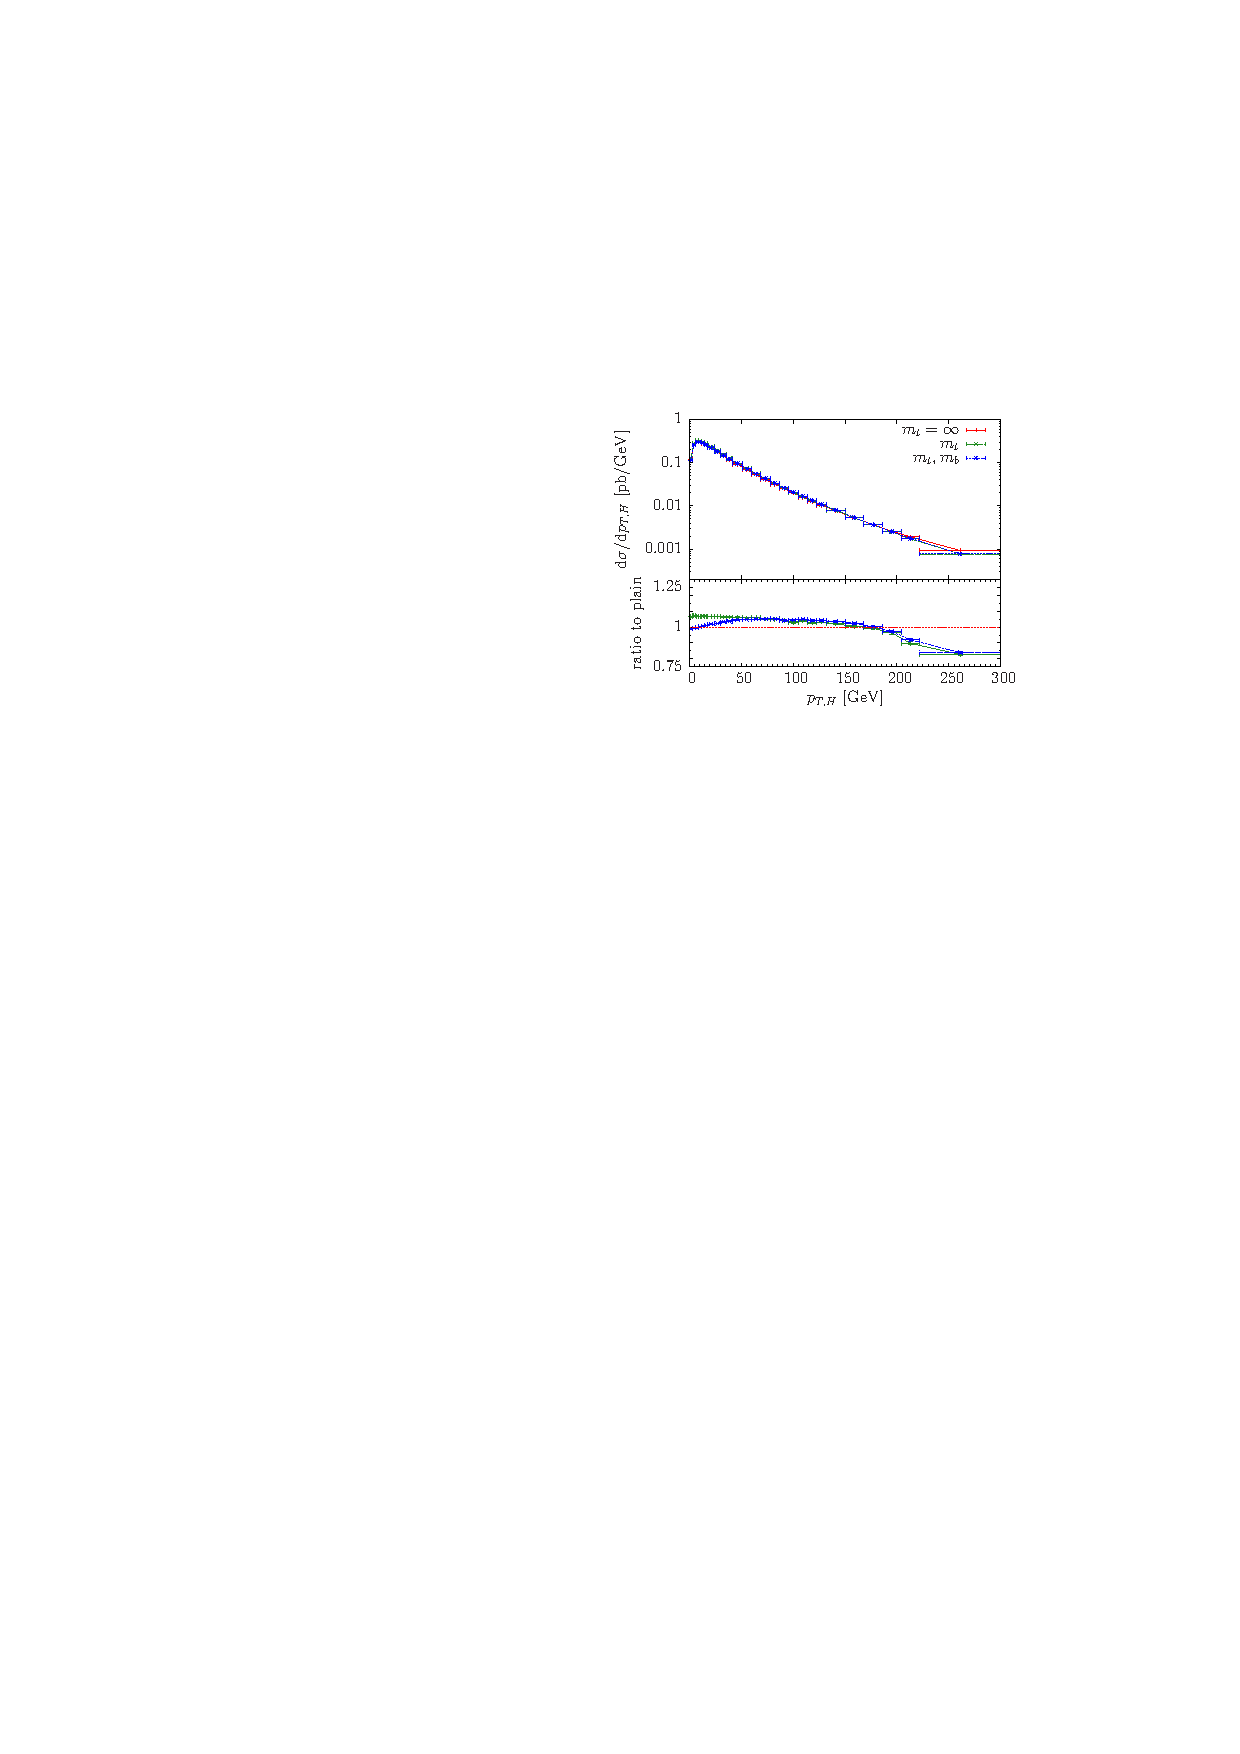
\includegraphics[width=0.6\linewidth]{img/theory/finitequarkmasseffects.pdf}
    \caption{
        The $\pth$ spectrum at $\sqrt{s}=8\TeV$ using the plain \textsc{HJ-MiNLO}~\cite{Hamilton:2015nsa} generator (red), and the same spectrum with finite quark mass effects due to the top quark (green) and the top and bottom quarks (blue).
        % 
        Taken from Ref.~\cite{Hamilton:2015nsa}.
        }
    \label{fig:finitequarkmasseffects}
  \end{center}
\end{figure}


In this thesis two particular calculations are considered, both computed up to NNLO and employing a resummation up to NNLL, and both investigating the properties of the $\pth$ spectrum under variations of the Higgs boson couplings.
% 
The first concerns an \textit{effective field theory}, in which the current SM Lagrangian is considered merely an effective low-energy Lagrangian; the actual effective Lagrangian is considered to contain higher-dimensional terms, that reduce to the SM Lagrangian only at low energy.
% 
Furthermore, the effective Lagrangian must have the same symmetries as present in the current SM Lagrangian~\cite{Grzadkowski:2010es}.
% 
To first approximation, one adds \textit{dimension-6 operators} to the SM Lagrangian:
% 
\begin{linenomath*}
\begin{equation}
\mathcal{L}_\text{eff} = \mathcal{L}_\text{SM} + \sum_i \frac{c_i}{\Lambda^2} \mathcal{O}_i
\,,
\end{equation}
\end{linenomath*}
% 
where $\mathcal{L}_\text{eff}$ is the effective Lagrangian, $\mathcal{O}$ a dimension-6 operator with corresponding coupling constant $c$, and $\Lambda$ is the scale at which these new physics effects become non-negligible (above the electroweak scale).
% 
In the model built in Refs.~\cite{Grazzini:2017szg,Grazzini:2016paz}, three dimension-6 operators are considered which, assuming a single Higgs production, can be expanded as
% 
\begin{linenomath*}
\begin{equation}
\frac{c_1}{\Lambda^2} \mathcal{O}_1 \to \frac{\alphas}{\pi v} \cg \hboson \, G^a_{\mu\nu} G^{a,\mu\nu}
\,,\quad 
\frac{c_2}{\Lambda^2} \mathcal{O}_2 \to \frac{m_\tquark}{v} \kappat \hboson \, \ttbar
\,,\quad 
\frac{c_3}{\Lambda^2} \mathcal{O}_3 \to \frac{m_\bquark}{v} \kappab \hboson \, \bbbar
\,.
\end{equation}
\end{linenomath*}
% 
The first term concerns a direct coupling of the Higgs field to the gluon field, which has the same underlying tensor structure as the calculation in the heavy top-mass limit.
% 
Its corresponding coupling constant $\cg$ is 0 in the SM.
% 
The second and third terms correspond to modifications of the coupling of the Higgs boson to top and bottom quarks.
% 
In this particular model, the inclusive cross section is approximately given by
% 
\begin{linenomath*}
\begin{equation}
\sigma \simeq \left| 12\cg + \kappat \right|^2 \sigma^\text{SM}
\,,
\end{equation}
\end{linenomath*}
% 
where the factor of 12 appears as a result of the definition of the corresponding dimension-6 operator~\cite{Grazzini:2016paz}.
% 
As first discussed in Ref.~\cite{Azatov:2013xha}, the shape of the $\pth$ distribution is able to break the degeneracy between $\cg$ and $\kappat$ in the inclusive cross section.
% 
A selection of calculations obtained from this model are shown in Fig.~\ref{fig:ktcgkb-precomputed}.


% The first is a model of simultaneous variations of $\kappat$, $\cg$, and $\kappab$ by adding dimension-6 operators to the SM Lagrangian, which has been built in Refs.~\cite{Grazzini:2017szg,Grazzini:2016paz}.
% % 
% % Hier verder, meer details over de daadwerkelijke dim 6 operators
% % 
% The dimension-6 operator whose coefficient is $\cg$ yields a direct coupling of the Higgs field to the gluon field with the same underlying tensor structure as in the heavy-top mass limit.
% % 
% In the SM, the value of $\cg$ equals 0.
% % 
% The introduction of $\cg$ in the effective Lagrangian is given in Ref.~\cite{Grazzini:2016paz} and the inclusive cross section is given by $\sigma \simeq \left| 12\cg + \kappat \right|^2 \sigma^\text{SM}$.
% % 
% Two other operators are included in the Lagrangian to describe modifications of the top and bottom Yukawa couplings with coefficients $\kappat$ and $\kappab$, respectively.
% % 
% Some precomputed spectra from Ref.~\cite{Grazzini:2017szg} are shown in Fig.~\ref{fig:ktcgkb-precomputed}.


\begin{figure}[hbtp]
  \begin{center}
    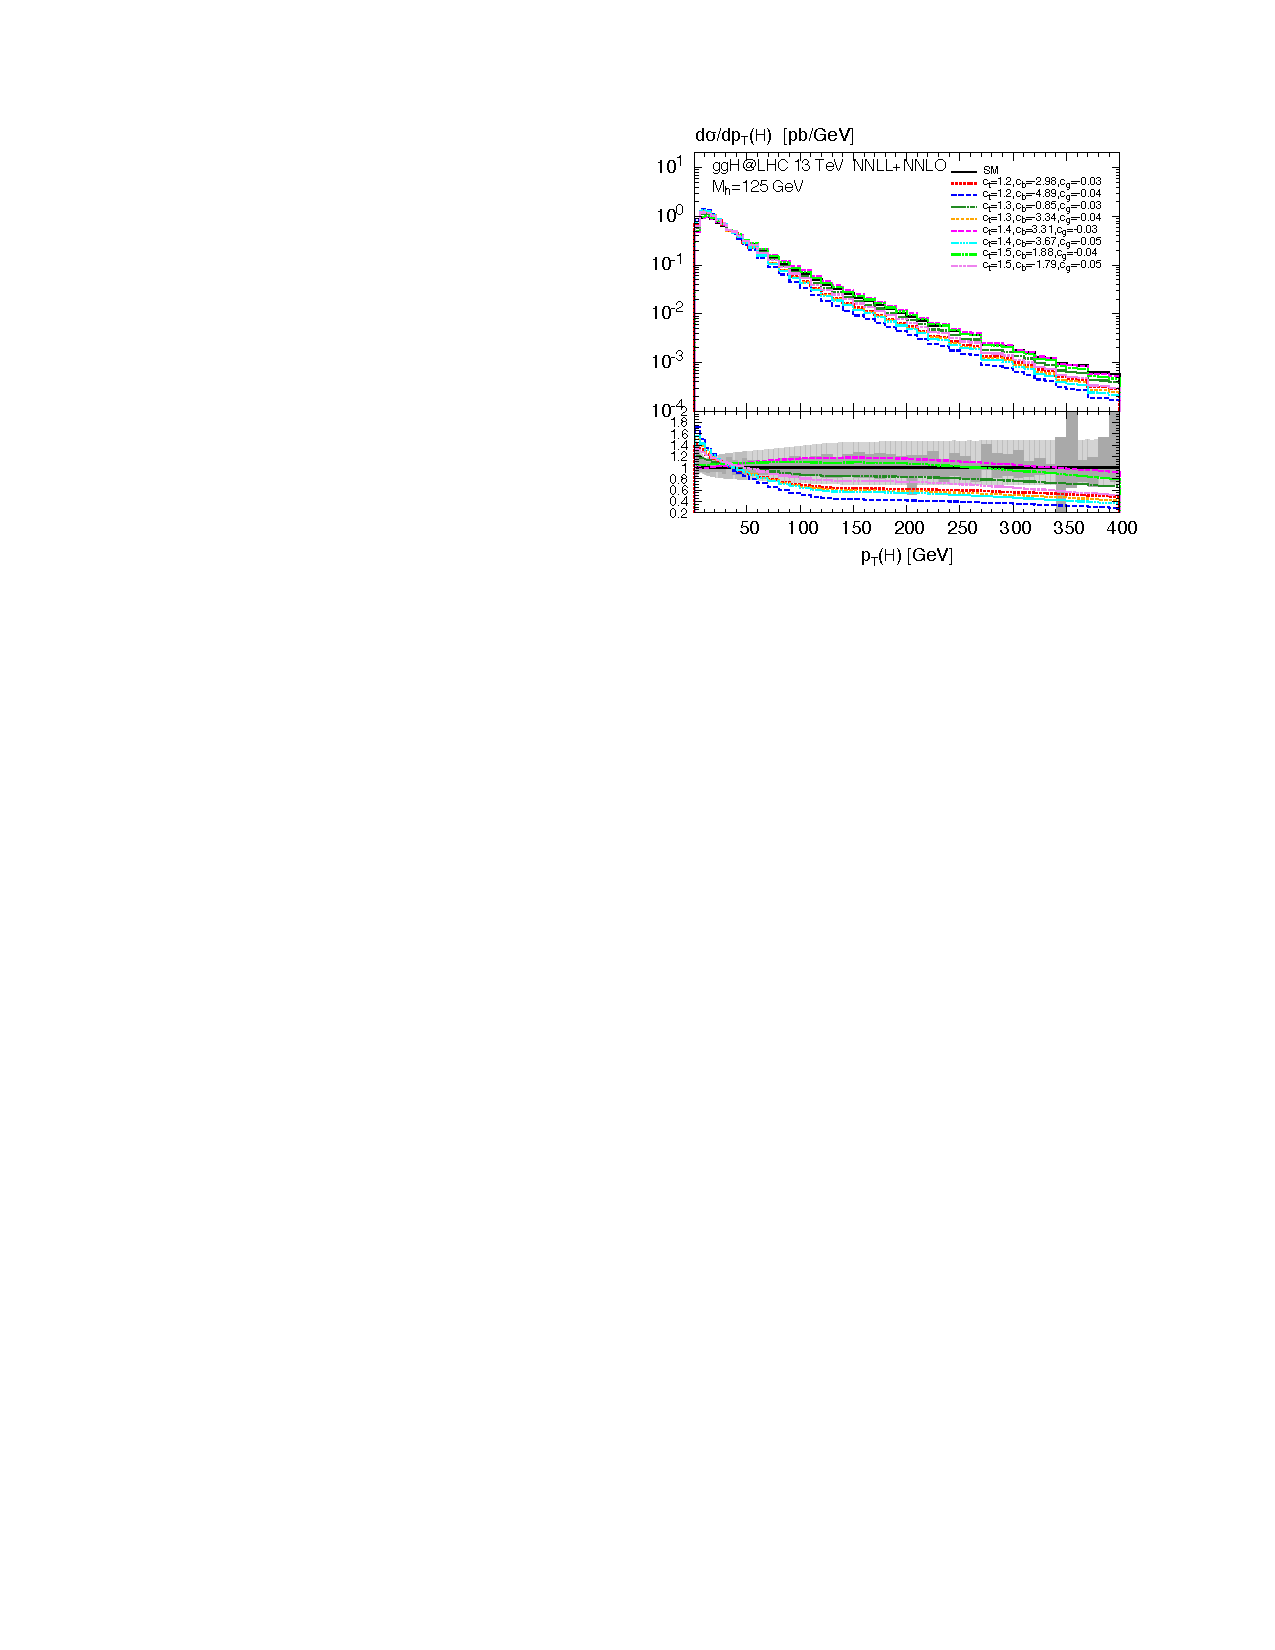
\includegraphics[width=0.6\linewidth]{img/theory/ktcgkb_variations.pdf}
    \caption{
        Selected $\pth$ spectra for various simultaneous variations of $\kappat$, $\cg$, and $\kappab$.
        % 
        The dark (light) band in the bottom part of the plot indicates the uncertainty due to missing higher order contributions in the NNLO+NNLL (NLO+NLL) calculation.
        % 
        Taken from Ref.~\cite{Grazzini:2017szg}.
        }
    \label{fig:ktcgkb-precomputed}
  \end{center}
\end{figure}


The second model~\cite{Bishara:2016jga} under consideration concerns variations of the Higgs boson couplings to lighter quarks, namely $\kappab$ and $\kappac$, while taking into account the interference of the top quark loop with that from the bottom and charm quarks in the gluon fusion production loop.
% 
Its calculation is also based on effective field theory, and has been made possible at NNLO+NNLL due to recent developments in resummation techniques~\cite{Bozzi:2003jy,Becher:2010tm,Monni:2016ktx}, and specific treatment of the mass corrections~\cite{Banfi:2013eda}.
% 
Some precomputed spectra from Ref.~\cite{Bishara:2016jga} are shown in Fig.~\ref{fig:kbkc-precomputed}.


\begin{figure}[hbtp]
  \begin{center}
    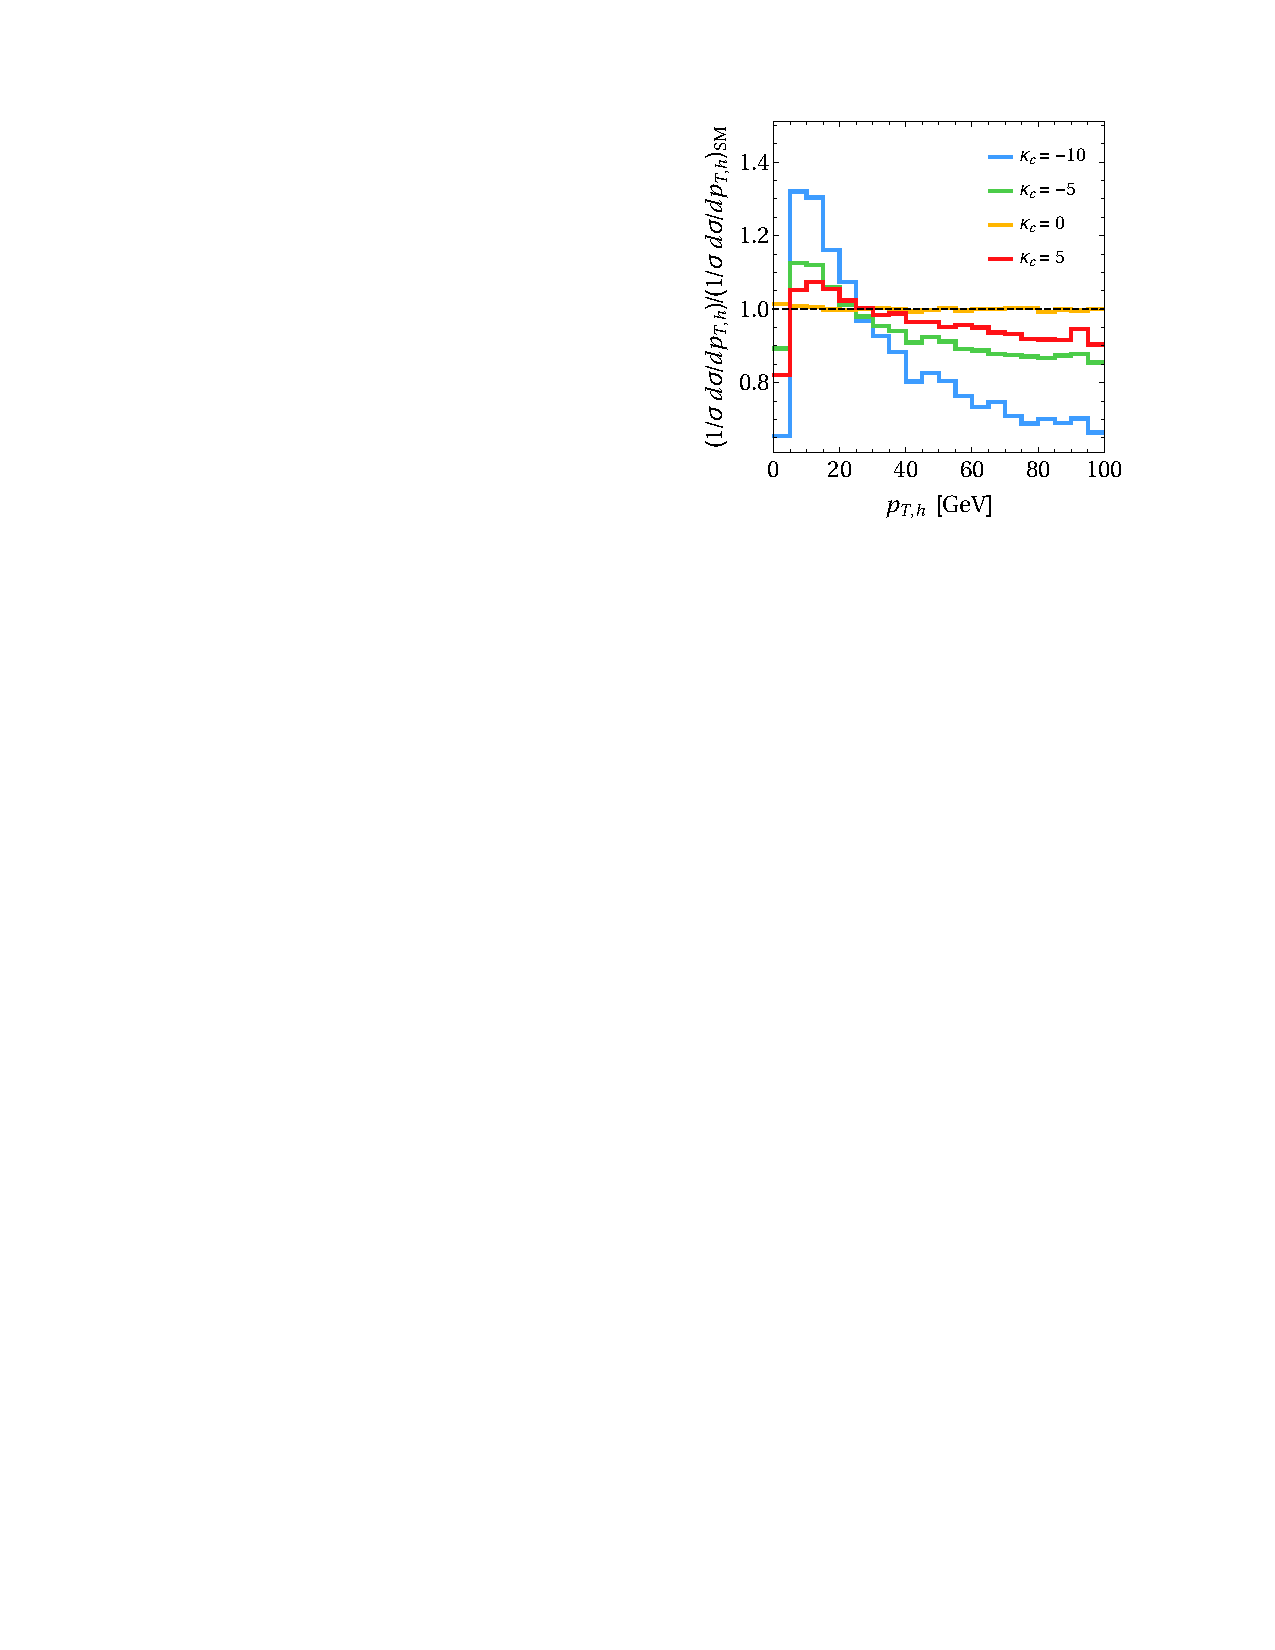
\includegraphics[width=0.6\linewidth]{img/theory/kbkc_variations.pdf}
    \caption{
        Normalized $\pth$ spectra for variations of $\kappac$, while $\kappab=1$.
        % 
        Taken from Ref.~\cite{Bishara:2016jga}.
        }
    \label{fig:kbkc-precomputed}
  \end{center}
\end{figure}



% ____________________________________________________________________________
\subsection{Simulation}

The theoretical aspects covered in this chapter are used as input in a simulation of particle physics data, which is ultimately what actual particle physics data is compared to derive measurements.
% 
Simulating proton-proton collisions is a complicated matter; the composition of the proton, the hard scattering interaction, and the parton showering and hadronization to ensure the color neutral final state all occur at different energy and time scales.
% 
These parts of the full particle physics event can be considered independent of one another, an idea termed the \textit{factorization theorem}.


Proton-proton interactions are actually interactions of the constituents of the proton, which are the \textit{valence quarks} (the quarks which give the proton its physical characteristics, such as its charge), \textit{sea quarks} (which originate from vacuum fluctuations), and gluons.
% 
When modeling a proton-proton interaction, one needs the individual momenta of these constituents; typically, this is expressed as the momentum fraction $x$ that the constituent carries with respect to the momentum of the full proton.
% 
The momentum-fraction distributions within the proton are called the \textit{parton distribution functions} (PDFs), which are derived from multivariate fits to data, mostly deep inelastic scattering and LHC data.
% 
The PDFs for the NNPDF3.1~\cite{Ball:2017nwa} PDF set are shown in Fig.~\ref{fig:nnpdf31}.


\begin{figure}[hbtp]
  \begin{center}
    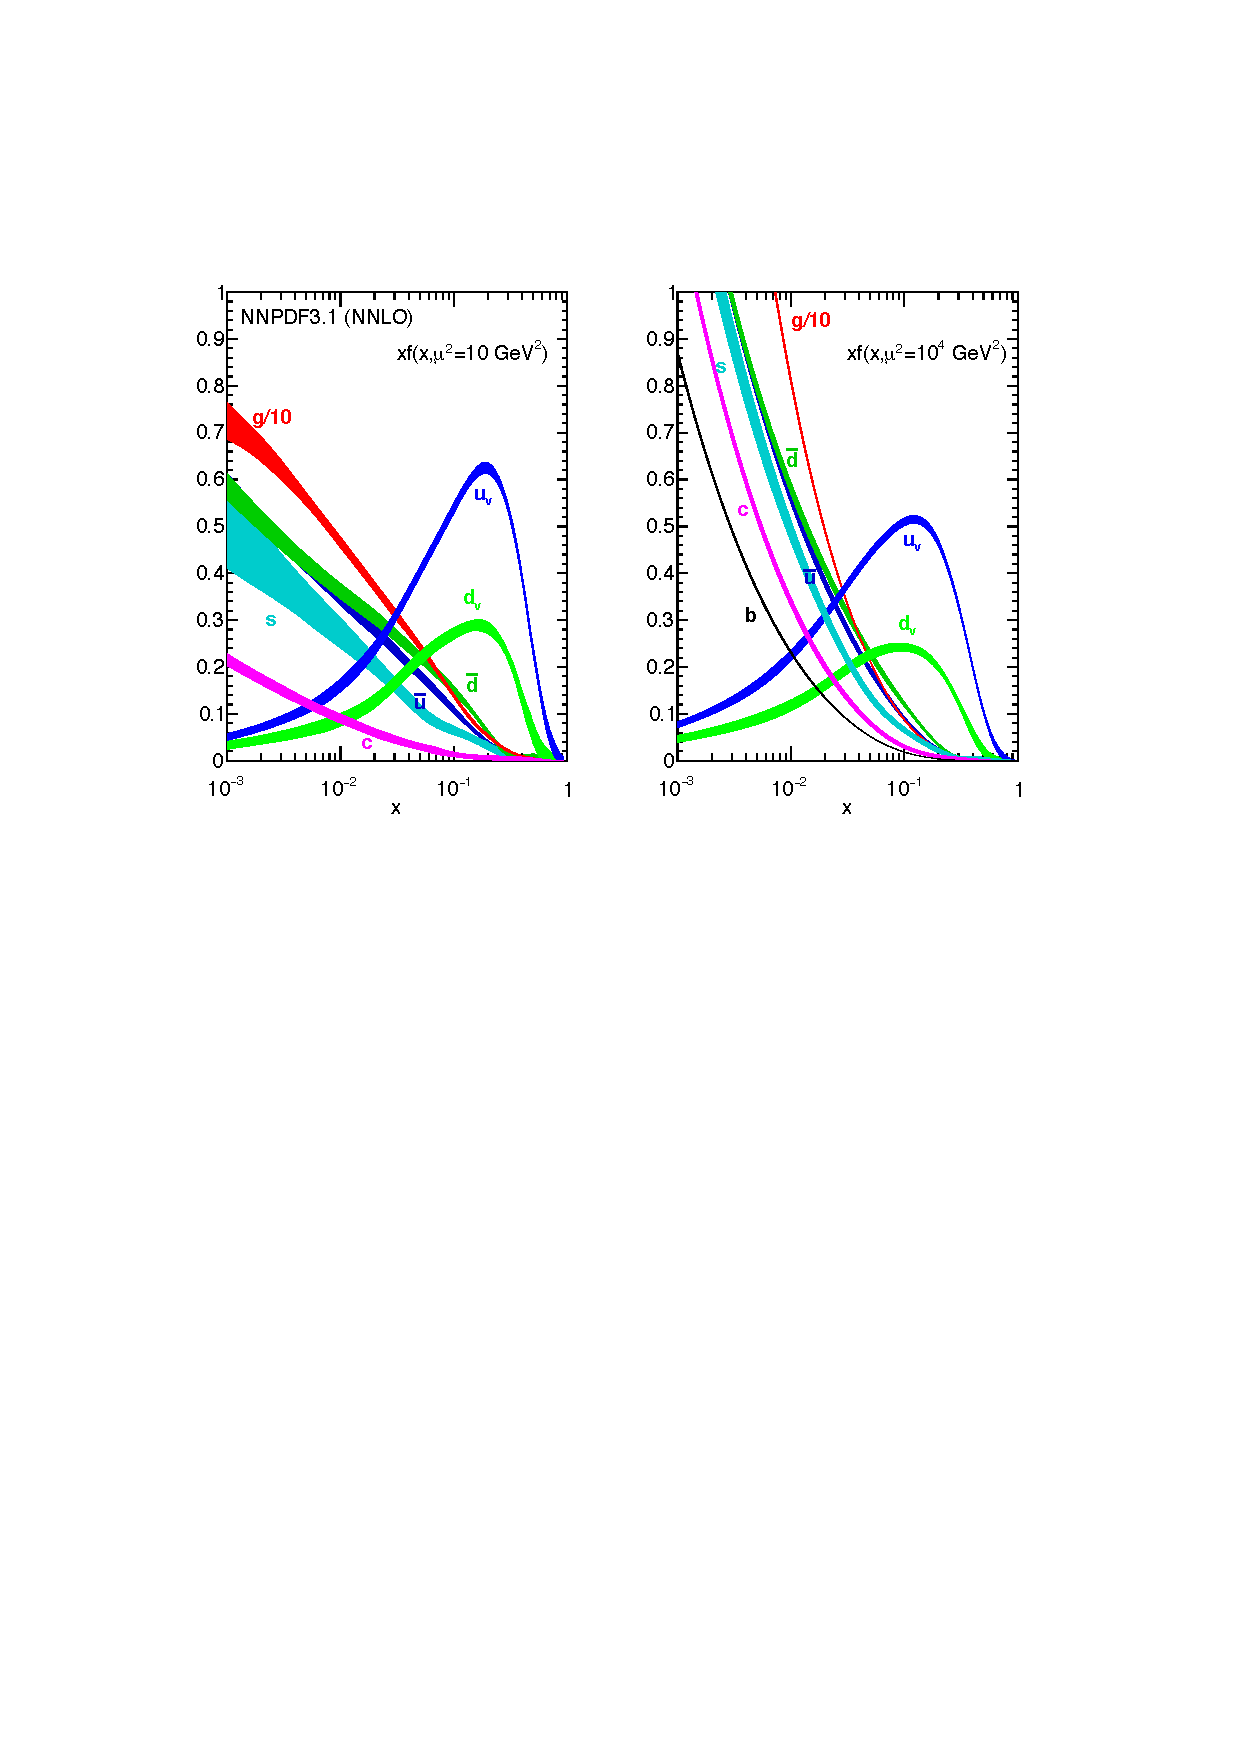
\includegraphics[width=0.6\linewidth]{img/theory/nnpdf31.pdf}
    \caption{
        The NNPDF3.1 PDFs at NNLO, at $\muR^2=\muF^2=10\GeV^2$ (left) and $\muR^2=\muF^2=10000\GeV^2$ (right).
        % 
        Taken from Ref.~\cite{Ball:2017nwa}.
        }
    \label{fig:nnpdf31}
  \end{center}
\end{figure}


Given the PDFs, the cross section of two protons going to any final state $X$ (not taking into account the parton showering and hadronization steps at the moment) can be written as
% 
\begin{linenomath*}
\begin{equation}
\sigma(\proton\proton\to X)
= \sum_{i,j} \int_0^1 \textrm{d}x_1 \int_0^1 \textrm{d}x_2
    \, \text{PDF}_i(x_1,\muF^2) \, \text{PDF}_j(x_2,\muF^2)
    \, \hat{\sigma}_{ij\to X}(x_1 p_1, x_2 p_2, \muR^2, \muF^2)
\,,
\end{equation}
\end{linenomath*}
% 
where the sum over $i$ and $j$ is a sum over all the possible combinations of initial-state partons carrying respective momentum fractions $x_1$ and $x_2$, and $\hat{\sigma}_{ij\to X}$ is the cross section of the hard interaction, given by theoretical calculation.
% 
The final state $X$ of the hard interaction part is typically not color neutral; as discussed in Section~\ref{sec:qcd}, colored particles evolve to color neutral final products, typically hadrons.
% 
This process is modeled in two steps: The first, called the \textit{parton shower}, concerns the hard QCD radiation of other particles, which is governed by perturbative QCD.
% 
As the partons radiate, the energy per particle decreases, until the point where the description given by pQCD breaks down, and the particles start to form color-neutral hadrons.
% 
This second step is called the \textit{hadronization}.
% 
Finally, in order to fully simulate real conditions, the \textit{underlying event} must be taken into account, which consists of the (typically) hadronic activity from the partons that were not part of the hard interaction.


The SM prediction for the differential cross sections in this thesis is simulated with $\MGvATNLO$ v2.2.2~\cite{Alwall:2014hca} for each of the four most prominent Higgs boson production modes ($\ggh$, VBF, VH, and $\tth$).
% 
The matrix element calculation is performed at NLO accuracy in perturbative QCD and includes the emission of up to two additional quarks or gluons.
% 
The parton showering and hadronization steps are performed using \PYTHIA8.205~\cite{Sjostrand:2014zea}, which is tuned with CUETP8M1~\cite{Skands:1695787} to take the underlying event into account.
% 
As the parton showering concerns QCD emissions much like the emissions already included in the matrix element calculation, one must be careful not to introduce any double counting; this is done by following the prescription in Ref.~\cite{Frederix:2012ps}.
% 
The predictions from the {\textsc{nnlops}} program~\cite{Hamilton:2012np, Kardos:2014dua} are considered to be the best for differential spectra, and as such simulated $\ggh$ events are weighted depending on $\pth$ and $\njets$ in order to match these predictions.
% 
This weighting procedure is discussed in Ref.~\cite{Sirunyan:2018koj}.
% 
Throughout the chain of simulation, the NNPDF3.0~\cite{Ball:2014uwa} PDF set is used.
% 
The anti-$\kt$ clustering algorithm~\cite{Cacciari:2008gp} is used on the stable particles of the hadronization step to create jets, using a distance parameter of $0.4$.


% \tk{TODO, paper text:} The SM prediction for the differential cross sections is simulated with $\MGvATNLO$ v2.2.2~\cite{Alwall:2014hca} for each of the four dominant Higgs boson production modes: gluon-gluon fusion (\ggh), vector boson fusion, associated production with a $\wboson$/$\zboson$ boson, and associated production with a top quark-antiquark pair.
% % 
% A contribution from Higgs boson production in association with bottom quarks is not simulated, but included assuming its acceptance is equal to that from Higgs boson production via gluon fusion.
% % 
% The matrix element calculation includes the emission of up to two additional partons and is performed at NLO accuracy in perturbative quantum chromodynamics (QCD).
% % 
% Events are interfaced to \PYTHIA8.205~\cite{Sjostrand:2014zea} for parton showering and hadronization with the CUETP8M1~\cite{Skands:1695787} underlying event tune.
% % 
% The matrix element calculation is matched to the parton shower following the prescription in Ref.~\cite{Frederix:2012ps}.
% % 
% A weight depending on $\pth$ and $\njets$ is applied to simulated $\ggh$ events to match the predictions from the {\textsc{nnlops}} program~\cite{Hamilton:2012np, Kardos:2014dua}, as discussed in Ref.~\cite{Sirunyan:2018koj}.
% % 
% The set of parton distribution functions used in all simulations is NNPDF3.0~\cite{Ball:2014uwa}.
% %
% The hadronic jets are clustered from the particle-flow candidates~\cite{Sirunyan:2017ulk} in the case of data and simulation, and from stable particles excluding neutrinos in the case of generated events, using the anti-$\kt$ clustering algorithm~\cite{Cacciari:2008gp} with a distance parameter of $0.4$.
% %
% The measurements are reported in terms of kinematic observables defined before the decay of the Higgs boson, i.e. at the generator level.

